\documentclass[preprint,12pt,a4paper]{elsarticle}
\usepackage[T1]{fontenc}
\usepackage{lmodern}
\usepackage[utf8]{inputenc}
\usepackage{amsmath,amssymb,amsthm}
\usepackage{booktabs,tabularx,multirow}
\usepackage{microtype}
\usepackage{algorithm}
\usepackage{algpseudocode}
\usepackage{xcolor}
\usepackage{graphicx}
\usepackage{tikz}
\usetikzlibrary{arrows.meta,positioning,fit,calc,backgrounds,shapes.geometric,shapes.multipart,decorations.pathreplacing}
\usepackage[hidelinks]{hyperref}
\usepackage{cleveref}

\newtheorem{theorem}{Theorem}
\newtheorem{lemma}{Lemma}
\newtheorem{corollary}{Corollary}
\newtheorem{proposition}{Proposition}
\theoremstyle{definition}
\newtheorem{definition}{Definition}
\newtheorem{example}{Example}
\newtheorem{assumption}{Assumption}
\theoremstyle{remark}
\newtheorem{remark}{Remark}
\crefname{assumption}{Assumption}{Assumptions}

\newcommand{\name}{DyFHL-PA}
\newcommand{\permit}{\mathsf{permit}}
\newcommand{\deny}{\mathsf{deny}}
\newcommand{\dec}{\mathrm{dec}}
\newcommand{\obo}{\mathsf{obo}}
\newcommand{\svc}{\mathsf{svc}}
\newcommand{\reads}{\mathrm{reads}}
\newcommand{\sinks}{\mathrm{sinks}}
\newcommand{\ident}{\mathrm{id}}
\newcommand{\Gap}{\mathrm{Gap}}
\newcommand{\Amp}{\mathrm{Amp}}
\newcommand{\Viol}{\mathrm{Viol}}
\newcommand{\Drift}{\mathrm{Drift}}
\newcommand{\Conf}{\mathrm{Conf}}
\newcommand{\Red}{\mathrm{Red}}
\newcommand{\Reg}{\mathrm{Reg}}
\newcommand{\F}{\mathcal{F}}
\newcommand{\G}{\mathcal{G}}
\newcommand{\Acc}{\mathcal{A}}
\newcommand{\key}{\mathrm{K}}
\newcommand{\Fp}{\mathbb{F}_p}
\newcommand{\shr}[1]{[\![#1]\!]}
\newcommand{\awsEvents}{1,089}
\newcommand{\awsMod}{874}
\newcommand{\awsAdd}{215}
\newcommand{\awsBasePol}{1,473}
\newcommand{\awsBaseSt}{7,475}
\newcommand{\awsUniverse}{12,599}
\newcommand{\awsGain}{958}
\newcommand{\awsLose}{23}
\newcommand{\awsMut}{629}
\newcommand{\awsRegMed}{2.1}
\newcommand{\awsRegMean}{7.7}
\newcommand{\awsRegNinety}{28.3}
\newcommand{\awsRegMax}{99.8}
\newcommand{\awsRegUnderOne}{39}
\newcommand{\awsRegUnderFive}{67}
\newcommand{\awsPolMed}{8.7}
\newcommand{\awsPolNinety}{62.2}
\newcommand{\awsLocViol}{0}
\newcommand{\awsRedEv}{22}
\newcommand{\awsRedPairs}{25}
\newcommand{\awsOvEv}{42}
\newcommand{\awsOvPairs}{559}
\newcommand{\awsAgentEv}{135}
\newcommand{\awsJobEv}{48}
\newcommand{\awsAgentPol}{69}
\newcommand{\awsAmpEv}{62}
\newcommand{\awsAmpROEv}{26}
\newcommand{\awsAmpROAct}{4,591}
\newcommand{\awsAmpVOEv}{29}
\newcommand{\awsHeld}{93}
\newcommand{\awsHeldPct}{8.5}
\newcommand{\awsChangedMed}{11}
\newcommand{\awsIncMs}{0.08}
\newcommand{\awsIncNinetyNine}{8.5}
\newcommand{\awsFull}{0.15}
\newcommand{\awsSecKBMed}{26.8}
\newcommand{\awsSecKBNinety}{5293}
\newcommand{\awsSecMBMax}{17.9}
\newcommand{\awsSecFullMBMed}{5.5}
\newcommand{\awsTopPol}{AIDevOpsAgentActionsPolicy}
\newcommand{\awsTopDate}{2026-08-19}
\newcommand{\awsTopAct}{4,409}
\newcommand{\eOneEvents}{3,000}
\newcommand{\eOneMism}{0}
\newcommand{\eOneSP}{140}
\newcommand{\eOneSPok}{140}
\newcommand{\eOneSC}{1,217}
\newcommand{\eOneSCok}{1,217}
\newcommand{\heldAll}{42}
\newcommand{\scBigRules}{25,669}
\newcommand{\scBigFull}{10.6}
\newcommand{\scBigMed}{13.6}
\newcommand{\scBigPnn}{228}
\newcommand{\scBigSpeed}{235}
\newcommand{\scBigReg}{0.0057}
\newcommand{\secMidFull}{91.3}
\newcommand{\secMidMean}{64}
\newcommand{\secMidMed}{6.4}
\newcommand{\secBigFull}{690}
\newcommand{\secBigMean}{392}
\newcommand{\secBigPnf}{2336}
\newcommand{\leakClasses}{160}
\newcommand{\leakDenied}{93}
\newcommand{\leakProbes}{222}
\newcommand{\leakEntropy}{95}
\newcommand{\leakRes}{90}
\newcommand{\exactRuns}{15}
\newcommand{\rkFed}{0.719}
\newcommand{\rkCount}{0.702}
\newcommand{\rkPool}{0.791}
\newcommand{\rkFedNew}{0.682}
\newcommand{\rkFedSeen}{0.727}
\newcommand{\rkCountSeen}{0.689}
\newcommand{\rkSeeds}{5}
\newcommand{\rkProp}{0.708}
\newcommand{\csTools}{229,827}
\newcommand{\csServers}{13,120}
\newcommand{\csOpen}{10,712}
\newcommand{\csOpenPct}{4.7}
\newcommand{\csRes}{59,169}
\newcommand{\csResPct}{25.7}
\newcommand{\csSrvOpen}{3,724}
\newcommand{\csSrvOpenPct}{28}


\journal{Computers \& Security}

\begin{document}
\begin{frontmatter}
\title{\name: Governing Change in Cross-Organisation Agent and Tool Ecosystems with Federated Dynamic Policy Hypergraphs}

\author[riadi]{Mokhtar Sellami\corref{cor}}
\cortext[cor]{Corresponding author.}
\address[riadi]{RIADI Laboratory, National School of Computer Science (ENSI), University of Manouba, Manouba, Tunisia}

\begin{abstract}
AI agents now reach the services and data platforms of several organisations through tools such as Model Context Protocol servers. Each owner governs only its own step of a call: who may invoke a tool, which identity may read a resource, and how the data may be used afterwards. These policies and the tools' own descriptions change continually, yet whether their composition remains governed is visible to no single owner, and none will disclose its policies to find out. We present \name, which treats governance as an invariant that every change must preserve. Rules of all owners and layers, tool descriptions and agent requests are hyperedges of one federated dynamic hypergraph, held in fragments by their owners. We define six cross-owner anomalies (conflict, redundancy, blocked grant, privilege amplification, usage violation and drift), prove that a change can alter findings only inside a region fixed by the vertices it touches, and derive an admission check that is necessary and sufficient for the invariant to hold after every change. The check runs across owners on secret shares: rule comparisons become inner products of incidence rows, and cross-layer checks reduce to products of bits that each owner computes from its own policy, so that owners learn only the findings addressed to them. A federated hyperedge model ranks held changes by expected use. On one year of AWS managed-policy history (\awsEvents{} changes) the region of a change is a median \awsRegMed\% of all statements, no finding changed outside it, and \awsAmpROEv{} changes would have given agent-facing policies \awsAmpROAct{} state-changing actions beyond the read-only job function. On constructed federations, admission agrees with full recomputation on \eOneEvents{} events and takes \scBigMed~ms (median) at \scBigRules{} rules, against \scBigFull~s for recomputation.
\end{abstract}


\begin{keyword}
access control \sep usage control \sep policy analysis \sep AI agents \sep Model Context Protocol \sep secure multi-party computation \sep hypergraphs \sep change management
\end{keyword}

\end{frontmatter}

%=====================================================================
\section{Introduction}\label{sec:intro}

% Plan: the setting and why it is new: agents cross organisational boundaries through tools; every step has its own owner.
Software agents built on large language models increasingly act on behalf of people by calling tools, and the Model Context Protocol (MCP) has become a common way to expose those tools~\cite{mcp2025spec,hou2026mcp}. A single request may involve a person in one organisation, an agent platform operated by a second, a tool hosted by a third and a data platform owned by a fourth. Each of them governs its own step: the agent platform decides who may call which tool, the data platform decides which identity may read which resource, and the data owner decides for which purpose and towards which destination the data may be used. These decisions are written by different people, in different languages, and they change continually: tools are added and re-described, rules are edited, usage terms are tightened, and agents delegate to other agents.

% Plan: why it is hard; state the open issues documented in 2026.
Recent analyses agree that this composition is poorly governed. The authentication and authorisation of MCP lacks a standard framework across clients and servers~\cite{hou2026mcp}, authorisation is optional in the protocol and often absent in implementations~\cite{nsa2026mcp}, and current identity patterns serve one agent inside one trust domain rather than chains across domains~\cite{openid2025agentic}. Tool descriptions change after they were approved~\cite{bharti2026drift} and can carry instructions that steer agents~\cite{wang2026mcptox}. A recent survey of agent authorisation lists as open the mapping of one organisation's policy onto another's, re-approval when tools change, and attenuation along delegation chains~\cite{surapani2026authz}. Underneath these reports lies a problem that policy analysis has not addressed: \emph{whether the policies of several owners, taken together, still govern every call after each change, when no owner may see the others' policies.}

% Plan: why existing tools do not solve it.
Existing policy analysers answer a different question. They take one readable policy set and check it for conflicts, redundancies or properties~\cite{fisler2005margrave,hu2013anomalies,lin2010exam,backes2018zelkova,barnett2025authz,cutler2024cedar}. Work on multi-domain policies integrates or reconciles policies that are disclosed to an integrator~\cite{bonatti2002algebra,mazzoleni2008integration,mcdaniel2006reconciliation}. Privacy-preserving analyses exist for firewall rules and role constraints between two domains~\cite{chen2013firewall,liu2020smer} and for the evaluation of one request against several owners' policies~\cite{sheikhalishahi2019multiparty}, but none of them covers tools, usage terms, delegation or change. Re-running a global analysis after every change is also not an option: it is quadratic in the number of rules, it requires the very disclosure that owners refuse, and deciding even whether one layer covers every request is coNP-complete (Theorem~\ref{thm:hard}).

% Plan: our idea in one paragraph.
This paper takes a different view. Governance is an \emph{invariant} of the joint state, and the object to check is the \emph{change}. We model the rules of all owners and layers, the tool descriptions and the agent requests as hyperedges of one hypergraph over shared attribute-value vertices. The hypergraph is \emph{federated}, because each owner holds its own fragment, and \emph{dynamic}, because every modification is an event on it. A change can only affect the findings that involve the vertices it touches, so its consequences can be computed exactly in a small region, by the owners of that region only, on secret shares. We call the approach \name.

% Plan: contributions as bullets with forward references.
\paragraph{Contributions}
\begin{enumerate}
\item \textbf{Model.} A federated dynamic policy hypergraph that represents tool, data and usage rules of several owners, tool descriptions with their approved and current versions, agent requests and delegation chains in one structure (Section~\ref{sec:model}).
\item \textbf{Invariant and anomalies.} Six cross-owner anomalies, a duality between blocked grants and amplifications that holds for any combining function, attenuation along chains, and the hardness of universal coverage (Section~\ref{sec:model}).
\item \textbf{Admission of change.} A locality theorem that bounds the effect of every event to a vertex region, and an admission check proved necessary and sufficient for preserving the invariant, with a commutation result for concurrent events (Section~\ref{sec:admission}).
\item \textbf{Flags-only protocol.} A two-server secret-sharing protocol in which same-layer checks are inner products of incidence rows and cross-layer checks are products of bits computed by each owner on its own policy; a simulation-based security statement with an explicit leakage function, and an analysis of what the findings themselves reveal (Section~\ref{sec:protocol}).
\item \textbf{Ranking.} A federated hyperedge model that orders held changes by the expected use of the requests they affect (Section~\ref{sec:ranking}).
\item \textbf{Evaluation} on one year of real AWS managed-policy changes, 229,827 real MCP tool schemas, constructed multi-organisation federations, three benchmarks of an earlier sketch-based design, and real access requests (Section~\ref{sec:evaluation}).
\end{enumerate}

% Plan: main findings, honestly stated.
\paragraph{Main findings} On the AWS history, the region of a change covers a median of \awsRegMed\% of all statements, and in \awsEvents{} changes no finding appeared or disappeared outside it. Admission would have held \awsHeld{} changes (\awsHeldPct\%), among them \awsAmpROEv{} that gave agent-facing policies state-changing actions not held by the read-only job function, \awsAmpROAct{} actions in total. On constructed federations, incremental admission is exact on \eOneEvents{} random events, and every one of the \eOneSP{} pairwise and \eOneSC{} cross-layer secure checks reveals exactly the plaintext findings. The learned ranking helps only where partners know a resource that the organisation does not: AUROC \rkFedNew{} against 0.5 on such resources, and no gain on known ones. Section~\ref{sec:discussion} states what the approach does not do.

\paragraph{Organisation} Section~\ref{sec:related} positions the work. Section~\ref{sec:setting} gives the running example, the system and threat model and the problem statement. Sections~\ref{sec:model} to~\ref{sec:ranking} present the model, the admission of change, the protocol and the ranking. Section~\ref{sec:evaluation} reports the evaluation, Section~\ref{sec:discussion} discusses deployment and limitations, and Section~\ref{sec:conclusion} concludes.

%=====================================================================
\section{Related work}\label{sec:related}

% Plan: theme 1 — analysis of one readable policy set; compare: single owner, no tools/usage, change only as diff of one policy.
\paragraph{Analysis of a single policy set} Policy analysis has a long tradition of checking one policy set that the analyser can read. Margrave compiles XACML policies to decision diagrams, verifies properties and computes the semantic difference between two versions~\cite{fisler2005margrave}. EXAM supports the comparison and integration of policies~\cite{lin2010exam}, and Hu et al.\ partition the request space into segments to find and resolve conflicts and redundancies in XACML~\cite{hu2013anomalies}, following the anomaly taxonomy introduced for distributed firewalls~\cite{alshaer2004firewalls}. For cloud policies, Zelkova encodes AWS policies in SMT~\cite{backes2018zelkova}, a formal model of the AWS authorisation engine covers identity-, resource- and organisation-level policies together~\cite{barnett2025authz}, and Cedar was designed so that its policies can be analysed~\cite{cutler2024cedar}. Bertino et al.\ organise the quality of policies into dimensions such as consistency, minimality, relevance and completeness~\cite{bertino2018quality}. These tools are exact and mature. They differ from our setting in three respects: they assume that one party can read all policies, they analyse one layer of decisions rather than the chain from tool to data to usage, and, where they handle change, they compare two versions of a single policy rather than checking the effect of one owner's change on findings that involve others. We reuse their core tests: our overlap and subsumption lemmas are the standard conditions for conjunctive rules.

% Plan: theme 2 — composition and multi-domain; compare: integrator sees policies; no change admission.
\paragraph{Composition and multi-domain policies} The algebra of Bonatti et al.\ composes policies of several authorities~\cite{bonatti2002algebra}; Gong and Qian study the complexity of secure interoperation between domains~\cite{gong1996interop}; Mazzoleni et al.\ integrate XACML policies of several parties~\cite{mazzoleni2008integration}; and McDaniel and Prakash show the limits of reconciling security policies~\cite{mcdaniel2006reconciliation}. More recently, John et al.\ derive leakage-free attribute-based policies for multi-cloud collaboration~\cite{john2026multicloud}. These works define how policies of different owners should combine, and we adopt one of their conclusions, that an action crossing owners should be allowed only if each owner allows its part. They assume, however, an integrator who reads the policies, and they compute a combined policy once rather than admitting changes to it.

% Plan: theme 3 — privacy-preserving policy analysis; compare closely (nearest prior work).
\paragraph{Privacy-preserving analysis across domains} Three lines of work analyse policies of several parties without disclosing them, and they are the closest to ours. Chen et al.\ remove redundant firewall rules across two administrative domains with a cooperative protocol in which neither firewall reveals its policy~\cite{chen2013firewall}. Liu et al.\ detect violations of separation-of-duty constraints between two role-based domains through a secure three-party matrix product~\cite{liu2020smer}. Sheikhalishahi et al.\ evaluate an access request against the policies of the co-owners of a resource with homomorphic encryption and secure function evaluation~\cite{sheikhalishahi2019multiparty}. Our same-layer check is closest to Liu et al.: comparing attribute rules also reduces to products of incidence matrices. We extend this to rules over several attributes and three anomaly types, add cross-layer checks between tool, data and usage policies, and restrict every computation to the region of a change. None of the three works models tools, delegation or usage terms, and none addresses change.

% Plan: theme 4 — change impact and incremental analysis.
\paragraph{Change and incremental analysis} Change-impact analysis computes which requests receive a different decision after an edit~\cite{fisler2005margrave}. Gofman et al.\ give incremental algorithms for user--role reachability under administrative role-based access control, deciding whether a change can affect the previous result and reusing it~\cite{gofman2010arbac}. Our locality theorem plays the same role for a federated, multi-layer state, and we add what an incremental analyser alone does not provide: a proof that checking the region of each change is necessary and sufficient for an invariant to hold in every reachable state, and a way to run that check across owners without disclosure.

% Plan: theme 5 — agent and MCP authorisation; compare: runtime enforcement vs static admission of policy change.
\paragraph{Authorisation for agents and tools} Usage control extends access control with obligations and conditions on use~\cite{park2004ucon}, and ODRL expresses such terms~\cite{w3c2018odrl}. For services and agents, zero-trust guidance places a policy decision at every hop~\cite{nist800207a}, token exchange carries the user on whose behalf a service acts~\cite{rfc8693}, and global authorisation services answer such checks at scale~\cite{pang2019zanzibar}. MCP specifies an OAuth-based authorisation flow but cannot enforce it at protocol level~\cite{mcp2025spec,nsa2026mcp}. Studies of the MCP ecosystem document missing authorisation~\cite{hou2026mcp}, tool poisoning~\cite{wang2026mcptox} and descriptions that change after audit~\cite{bharti2026drift}; a survey of agent authorisation lists re-approval on tool change and cross-organisation policy mapping as open~\cite{surapani2026authz}. This work addresses the enforcement of a decision at run time and the detection of malicious descriptions. Our question is complementary: whether the policies that the enforcement points apply remain jointly consistent as they change. The confused-deputy problem~\cite{hardy1988deputy} appears in our model as privilege amplification, a property of the composed policies rather than of a single call.

% Plan: theme 6 — hypergraph and federated learning, short.
\paragraph{Hypergraph and federated learning} Hypergraph neural networks propagate information between vertices through hyperedges~\cite{feng2019hgnn}, and federated averaging trains a shared model without pooling data~\cite{mcmahan2017fedavg}. We use both only for the optional ranking component, and our evaluation reports that hypergraph propagation does not improve over a hyperedge scorer.

% Plan: positioning table.
\Cref{tab:related} summarises the comparison. To our knowledge, no prior work admits changes to the policies of several owners across tool, data and usage layers with exact results and without disclosure.

\begin{table}[t]
\centering\footnotesize
\caption{Positioning. \emph{Owners}: policies of several owners analysed together; \emph{private}: no owner discloses its policy; \emph{layers}: tool, data and usage decisions composed; \emph{change}: effect of a change computed incrementally; \emph{exact}: no false alarms or misses by design. $\circ$: partially.}\label{tab:related}
\begin{tabularx}{\linewidth}{Xccccc}
\toprule
Work & Owners & Private & Layers & Change & Exact\\
\midrule
Margrave~\cite{fisler2005margrave} & -- & -- & -- & $\circ$ & \checkmark\\
Segment-based XACML analysis~\cite{hu2013anomalies}, EXAM~\cite{lin2010exam} & $\circ$ & -- & -- & -- & \checkmark\\
Zelkova~\cite{backes2018zelkova}, AWS engine model~\cite{barnett2025authz} & -- & -- & $\circ$ & -- & \checkmark\\
Policy integration~\cite{mazzoleni2008integration}, algebra~\cite{bonatti2002algebra} & \checkmark & -- & -- & -- & \checkmark\\
Incremental ARBAC analysis~\cite{gofman2010arbac} & -- & -- & -- & \checkmark & \checkmark\\
Cooperative firewall optimisation~\cite{chen2013firewall} & \checkmark & \checkmark & -- & -- & \checkmark\\
Secure SMER detection~\cite{liu2020smer} & \checkmark & \checkmark & -- & -- & \checkmark\\
Private multi-party evaluation~\cite{sheikhalishahi2019multiparty} & \checkmark & \checkmark & -- & -- & \checkmark\\
\name{} (this work) & \checkmark & \checkmark & \checkmark & \checkmark & \checkmark\\
\bottomrule
\end{tabularx}
\end{table}

%=====================================================================
\section{Setting and problem}\label{sec:setting}

\subsection{Running example}\label{sec:example}
% Plan: two organisations and three changes, used throughout.
A clinic $C$ owns two resources, electronic health records (\textit{ehr}) and insurance claims (\textit{claims}). A vendor $V$ operates an agent platform that $C$'s staff use, and hosts two MCP tools: \texttt{summarise}, which reads \textit{ehr} under a service account of $V$, and \texttt{export}, which reads \textit{claims} on behalf of the calling user and sends a report to $V$'s analytics store in the EU. $V$'s tool policy lets clinicians and analysts call \texttt{summarise} and analysts call \texttt{export}. $C$'s data policy lets clinicians read \textit{ehr} and analysts read \textit{claims}. $C$'s usage policy allows \textit{claims} to be used for analytics by $C$ or $V$ in the EU and to be retained for at most 30 days.

Three changes occur in one week.
\begin{description}
\item[$\epsilon_1$ (by $C$).] Users complain that \texttt{summarise} always fails, because $C$ never granted $V$'s service account access to \textit{ehr}. $C$ adds a data rule that does.
\item[$\epsilon_2$ (by $V$).] $V$ updates the description of \texttt{export}: reports are now also sent to a research partner $R$ in the US.
\item[$\epsilon_3$ (by $V$).] $V$ lets interns call \texttt{export}.
\end{description}
Each change is reasonable from its author's point of view, and each is reviewed by its author only. After $\epsilon_1$, analysts read health records through \texttt{summarise} that $C$ denies them directly. After $\epsilon_2$, claims leave the region and the organisations that $C$ allows. After $\epsilon_3$, interns are offered a tool that $C$'s policy will refuse. No owner sees any of these three facts in its own policy, and neither owner is willing to show its policy to the other. The rest of the paper shows how the three changes are detected at the moment they are made, by the owners concerned only, and without either owner reading the other's rules.

\subsection{System model}
% Plan: organisations, layers, tools, the shared vocabulary assumption.
A finite set $O$ of organisations shares an environment. Each organisation owns users, agents, tools and resources, writes the policies that govern what it owns, and runs policy enforcement points that apply them. A call by an agent crosses three decisions, which we call \emph{layers}.
\begin{itemize}
\item The \emph{tool layer} decides whether a user, through an agent, may invoke a tool. It belongs to the organisation that hosts the tool or operates the gateway in front of it.
\item The \emph{data layer} decides whether an identity may access a resource. It belongs to the owner of the resource.
\item The \emph{usage layer} decides for which purpose, towards which destination and for how long a resource may be used once read, in the sense of usage control~\cite{park2004ucon}. It belongs to the owner of the resource.
\end{itemize}
A tool is described by the resources it reads, its purpose, its retention, the destinations (\emph{sinks}) it sends to, and the identity under which it acts: the calling user (\emph{on behalf of}, as with token exchange~\cite{rfc8693}) or a service account of its host. A tool has an \emph{approved} description, recorded when an owner accepted it, and a \emph{current} one, which the tool publishes and may change.

\begin{assumption}[Shared vocabulary]\label{as:vocab}
The organisations agree on the attributes and values used to describe principals, tools, resources, purposes and sinks, or on a mapping between their vocabularies.
\end{assumption}
\begin{assumption}[Mediation]\label{as:mediation}
Every call passes the enforcement point of each layer, which receives the user, the agent, the tool and the effective identity.
\end{assumption}
\Cref{as:vocab} is what any cross-organisation policy needs, encrypted or not; we return to its cost in Section~\ref{sec:discussion}. \Cref{as:mediation} is the subject of zero-trust architectures~\cite{nist800207a}; we do not check it, we check what the enforcement points enforce.

\begin{figure}[t]
\centering
\resizebox{\linewidth}{!}{%
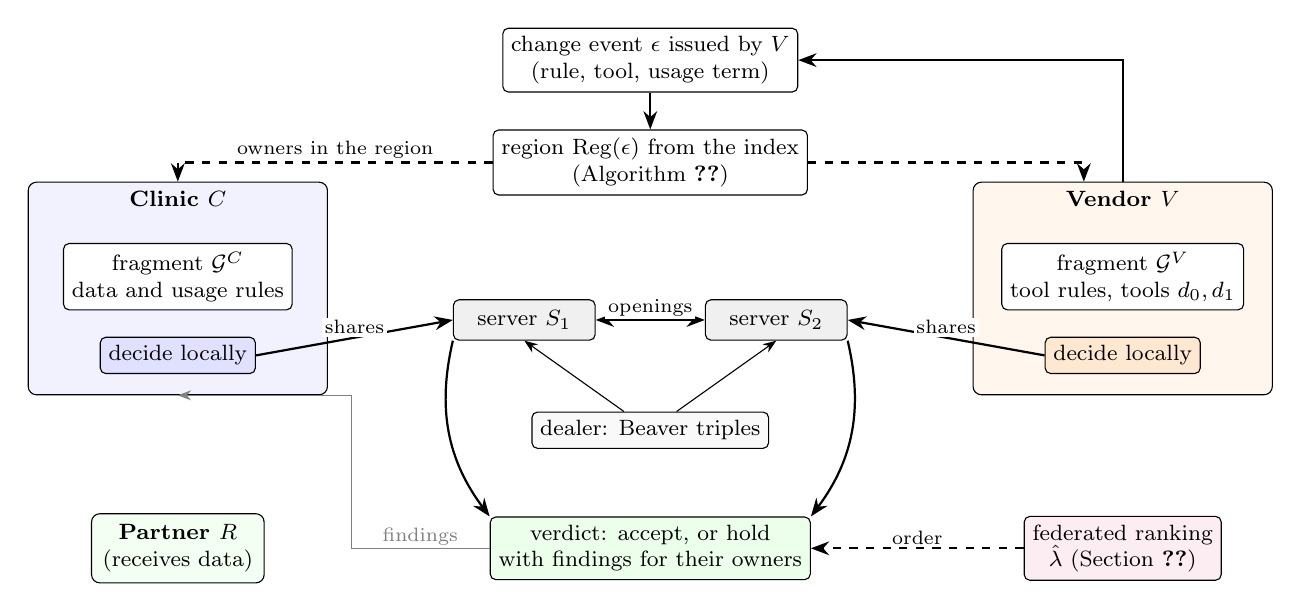
\begin{tikzpicture}[
  font=\footnotesize, >=Stealth,
  org/.style={draw, rounded corners=3pt, minimum width=3.8cm, minimum height=2.7cm},
  box/.style={draw, rounded corners=2pt, fill=white, align=center, inner sep=3pt},
  srv/.style={draw, fill=gray!12, rounded corners=2pt, align=center, minimum width=1.8cm, inner sep=4pt},
  lbl/.style={fill=white, inner sep=1pt, font=\scriptsize},
  arr/.style={->, thick}]
\node[org, fill=blue!5] (C) at (0,0.4) {};
\node[anchor=north, font=\footnotesize\bfseries] at (C.north) {Clinic $C$};
\node[box] (Cf) at (0,0.55) {fragment $\G^{C}$\\ data and usage rules};
\node[box, fill=blue!12] (Cl) at (0,-0.45) {decide locally};
\node[org, fill=orange!7] (V) at (12,0.4) {};
\node[anchor=north, font=\footnotesize\bfseries] at (V.north) {Vendor $V$};
\node[box] (Vf) at (12,0.55) {fragment $\G^{V}$\\ tool rules, tools $d_0, d_1$};
\node[box, fill=orange!18] (Vl) at (12,-0.45) {decide locally};
\node[box, minimum width=3.4cm] (ev) at (6,3.3) {change event $\epsilon$ issued by $V$\\ (rule, tool, usage term)};
\node[box, minimum width=3.4cm] (reg) at (6,2.0) {region $\Reg(\epsilon)$ from the index\\ (Algorithm~\ref{alg:region})};
\node[srv] (s1) at (4.4,0.0) {server $S_1$};
\node[srv] (s2) at (7.6,0.0) {server $S_2$};
\node[box, fill=gray!5] (deal) at (6,-1.4) {dealer: Beaver triples};
\node[box, fill=green!8, minimum width=3.4cm] (ver) at (6,-2.9) {verdict: accept, or hold\\ with findings for their owners};
\node[box, fill=purple!7] (rank) at (12,-2.9) {federated ranking\\ $\hat\lambda$ (Section~\ref{sec:ranking})};
\node[draw, rounded corners=3pt, fill=green!5, align=center, inner sep=4pt] (R) at (0,-2.9) {\textbf{Partner $R$}\\ (receives data)};
\draw[arr] (V.north) |- (ev.east);
\draw[arr] (ev) -- (reg);
\draw[arr, dashed] (reg.west) -| node[lbl, pos=0.25, above] {owners in the region} (C.north);
\draw[arr, dashed] (reg.east) -| (V.110);
\draw[arr] (Cl.east) -- node[lbl, above] {shares} (s1.west);
\draw[arr] (Vl.west) -- node[lbl, above] {shares} (s2.east);
\draw[<->, thick] (s1.east) -- node[lbl, above] {openings} (s2.west);
\draw[->] (deal) -- (s1.south); \draw[->] (deal) -- (s2.south);
\draw[arr] (s1.south west) to[bend right=25] (ver.north west);
\draw[arr] (s2.south east) to[bend left=25] (ver.north east);
\draw[arr, dashed] (rank) -- node[lbl, above] {order} (ver);
\draw[->, gray] (ver.west) -- node[lbl, above, text=gray] {findings} (R.east -| 2.2,-2.9) -- (2.2,-2.9) |- (C.south);
\end{tikzpicture}}
\caption{Architecture of \name. Each organisation holds its fragment of the policy hypergraph. A change event determines a region; only the owners of that region evaluate their own rules locally and send secret shares to two non-colluding servers, which combine them and return the findings to the owners they concern. A federated model ranks held changes by expected use.}\label{fig:arch}
\end{figure}

\subsection{Threat model}\label{sec:threat}
% Plan: semi-honest owners and servers, non-colluding servers, dealer, what is protected and what is revealed.
Owners and servers are \emph{honest but curious}: they follow the protocol and try to learn other owners' rules from what they see. Owners may collude with each other. The two servers do not collude with each other, and neither colludes with an owner; correlated randomness comes from a dealer, which may be replaced by a preprocessing protocol (Section~\ref{sec:cost}). The \emph{protected} information is the rule set of each owner. The \emph{revealed} information is fixed by a leakage function given in Section~\ref{sec:security}: the findings addressed to each owner, the descriptions of the tools that read a resource to the owner of that resource (which must see them to approve them), and the number of rules each owner holds on the vertices of a region. Malicious owners that submit malformed rules, denial of service, and the correctness of tool descriptions with respect to the tools' code are outside the model; drift between observed and declared behaviour is covered as an anomaly when observations exist.

\subsection{Problem statement}\label{sec:problem}
Let $\G_0$ be the joint state of all policies and tool descriptions and $\epsilon_1, \epsilon_2, \dots$ a sequence of change events, each issued by one owner.
\begin{description}
\item[P1, governance as an invariant.] Define anomalies of the composed policy that capture conflicting, superfluous, blocked, amplified, non-conforming and drifted authority, and an invariant stating that every anomaly present has been accepted by the owners it concerns.
\item[P2, admission of change.] For each event, decide before it takes effect whether the successor state satisfies the invariant, at a cost that depends on the event and not on the size of the state, exactly (no false alarms and no misses).
\item[P3, no disclosure.] Run the decision of P2 so that each owner learns only the findings that involve its own rules, tools or resources, and a stated leakage.
\item[P4, priority.] Order the held changes by the expected use of the requests they affect, without pooling request logs.
\end{description}

%=====================================================================
\section{The federated dynamic policy hypergraph}\label{sec:model}

\Cref{tab:notation} lists the notation used in the rest of the paper.

\begin{table}[t]
\centering\small
\caption{Notation.}\label{tab:notation}
\begin{tabularx}{\linewidth}{lX}
\toprule
$O$, $o$ & organisations (owners)\\
$\ell \in \{\mathsf{tool},\mathsf{data},\mathsf{usage}\}$ & layer; $A_\ell$ its attributes, $D_a$ the domain of attribute $a$\\
$e = (\ell, o, x, c, b)$ & rule: layer, owner, effect, condition, obligations; $M(e)$ its match set\\
$V$, $h(e)$ & vertices (attribute values and wildcards); hyperedge of rule $e$\\
$\key(e)$ & key vertices of $e$: the resources (data, usage) or tools (tool layer) it constrains\\
$\G = (E, d_0, d_1)$, $\G^o$ & joint state (rules, approved and current tool descriptions); fragment of owner $o$\\
$\dec_\ell$, $\kappa$ & decision of layer $\ell$; combining function\\
$d(t) = (\reads(t), p_t, \rho_t, \sinks(t), \beta_t)$ & tool description: reads, purpose, retention, sinks, binding\\
$\ident_\beta(u)$ & effective identity of a call by $u$ under binding $\beta \in \{\obo, \svc(c)\}$\\
$S$ & population of user attribute vectors (subject classes)\\
$\F(\G)$, $\Acc$ & findings of a state; findings accepted by their owners\\
$\epsilon$, $\G \oplus \epsilon$, $\Reg(\epsilon)$ & change event; successor state; region of the event\\
$\shr{x}$, $\Fp$ & additive secret sharing of $x$ over the field with $p = 2^{31}-1$\\
\bottomrule
\end{tabularx}
\end{table}

\subsection{Attributes, rules and hyperedges}
Each layer $\ell$ has a finite set $A_\ell$ of attributes, qualified by the entity they describe (\textit{usr.role}, \textit{tool.name}, \textit{res.id}, \textit{sink.region}), and each attribute $a$ has a finite domain $D_a$. Hierarchies, ranges and negated values are reduced beforehand to disjoint atoms, so that a condition on an attribute is a set of atoms. A \emph{request} of layer $\ell$ assigns one value to every attribute; $Q_\ell = \prod_{a \in A_\ell} D_a$.

\begin{definition}[Rule]\label{def:rule}
A rule is a tuple $e = (\ell, o, x, c, b)$ of a layer $\ell$, an owner $o \in O$, an effect $x \in \{\permit, \deny\}$, a condition $c$ mapping every $a \in A_\ell$ to a non-empty set $c(a) \subseteq D_a$, and a finite set $b$ of obligations. The rule matches $q \in Q_\ell$ when $q(a) \in c(a)$ for every $a$; its match set is
\begin{equation}
M(e) = \textstyle\prod_{a \in A_\ell} c(a). \label{eq:matchset}
\end{equation}
\end{definition}

\begin{definition}[Policy hypergraph]\label{def:hypergraph}
The vertex set $V$ has one vertex $(a, v)$ for every attribute $a$ and value $v \in D_a$, and one wildcard vertex $(a, \ast)$ per attribute. The hyperedge of a rule is
\[
h(e) = \{(a, v) : c(a) \neq D_a,\ v \in c(a)\} \cup \{(a, \ast) : c(a) = D_a\}.
\]
A request $q$ is the hyperedge $\{(a, q(a)) : a \in A_\ell\}$, and a tool description (\Cref{def:tool}) is the hyperedge of its tool, read resources, purpose and sinks.
\end{definition}
The wildcard gives a normal form: a condition that lists every value and one that leaves the attribute open denote the same match set and the same hyperedge. Without it the syntactic tests below are incomplete.

\begin{definition}[Key vertices]\label{def:key}
The key attribute of the data and usage layers is the resource, that of the tool layer is the tool. The key vertices $\key(e)$ of a rule are the values of $c$ on its key attribute.
\end{definition}
An owner can only govern what it owns, so a rule of owner $o$ constrains its key attribute to resources or tools owned by $o$, or co-owned with others in a shared scope. Key vertices are therefore never wildcards; this is what makes regions small (Section~\ref{sec:admission}).

\begin{definition}[Federated dynamic policy hypergraph]\label{def:fdph}
A state is $\G = (E, d_0, d_1)$, where $E$ is a finite set of rules and $d_0, d_1$ map every tool to its approved and current description. The \emph{fragment} of owner $o$ is $\G^o$: its rules $E^o = \{e \in E : e \text{ has owner } o\}$ and the descriptions of the tools it hosts. An \emph{event} is one of $\mathsf{ins}(e)$, $\mathsf{del}(e)$, $\mathsf{redesc}(t, d)$ and $\mathsf{approve}(t)$, issued by the owner of $e$ or the host of $t$; $\G \oplus \epsilon$ is the resulting state, with $\mathsf{approve}(t)$ setting $d_0(t) := d_1(t)$.
\end{definition}

\subsection{Decisions, identities and composition}
Let $E_\ell(q)$ be the rules of layer $\ell$ that match $q$. A \emph{combining function} $\kappa$ maps the effects of $E_\ell(q)$ to a decision, with $\kappa(\emptyset) = \deny$; deny-overrides, permit-overrides and first-applicable are common choices~\cite{oasis2013xacml}. Then $\dec_\ell(q) = \kappa(E_\ell(q))$. A resource co-owned by several organisations is decided on the union of their rules. All results below that concern decisions hold for every $\kappa$.

Users and service accounts are described by the same identity attributes; $I$ is the set of identity vectors and $S \subseteq I$ a population of user vectors, for instance all combinations of role, department and organisation. A tool-layer request is a pair $(u, t)$, a data-layer request a pair $(i, r)$, a usage-layer request a triple $(r, p, s)$ of a resource, a purpose and a sink.

\begin{definition}[Tool description]\label{def:tool}
A description
\[d(t) = (\reads(t), p_t, \rho_t, \sinks(t), \beta_t)\]
gives the resources the tool reads, its purpose, its retention, its sinks and its binding $\beta_t$, either $\obo$ or $\svc(c)$ for an identity $c \in I$. The effective identity of a call by $u$ is $\ident_{\obo}(u) = u$ and $\ident_{\svc(c)}(u) = c$.
\end{definition}

\begin{definition}[Composition]\label{def:composition}
A call of tool $t$ by user $u$ that reads $r \in \reads(t)$ is \emph{permitted by the composition} when $\dec_{\mathsf{tool}}(u, t) = \permit$, $\dec_{\mathsf{data}}(\ident_{\beta_t}(u), r) = \permit$, $\dec_{\mathsf{usage}}(r, p_t, s) = \permit$ for every $s \in \sinks(t)$, and $\rho_t \le \rho^{\max}(r)$, where $\rho^{\max}(r)$ is the retention bound set by the owner of $r$.
\end{definition}
The composition is a conjunction: every owner on the path must allow its part, which is the rule that the multi-domain literature arrives at~\cite{bonatti2002algebra,gong1996interop}.

\begin{example}\label{ex:model}
In the running example, $V$'s tool rule $e_1$ has $c(\textit{usr.role}) = \{\textit{clinician}, \textit{analyst}\}$, $c(\textit{tool}) = \{\texttt{summarise}\}$ and the wildcard elsewhere, so $\key(e_1) = \{\texttt{summarise}\}$. $C$'s data rule $e_3$ permits \textit{clinician} on \textit{ehr}. \texttt{summarise} has binding $\svc(c_V)$, where $c_V$ is $V$'s service account. Figure~\ref{fig:example} draws the state as an incidence graph.
\end{example}

\begin{figure}[t]
\centering
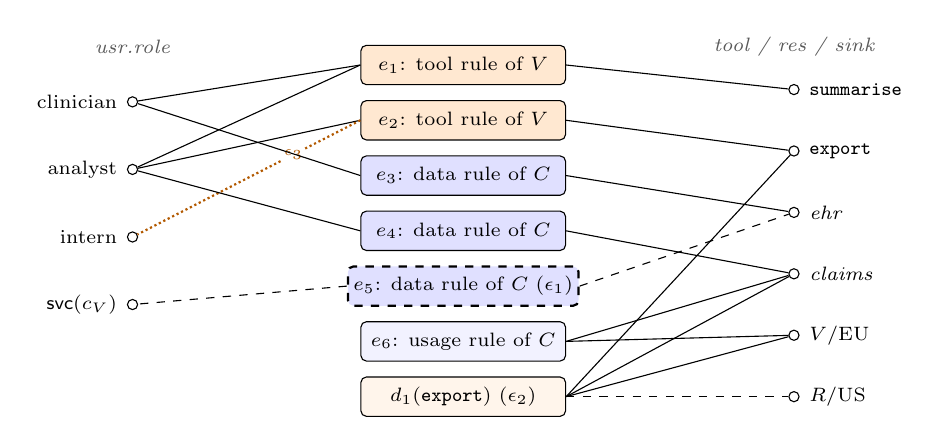
\begin{tikzpicture}[font=\scriptsize, >=Stealth, y=0.78cm,
  v/.style={circle, draw, fill=white, inner sep=1.3pt},
  he/.style={draw, rounded corners=2pt, inner sep=2pt, align=center, minimum width=2.6cm, minimum height=0.5cm},
  lab/.style={font=\scriptsize\itshape, text=gray!70!black}]
\node[lab] at (0,4.2) {usr.role};
\node[v, label=left:{clinician}] (sA) at (0,3.3) {};
\node[v, label=left:{analyst}] (sB) at (0,2.2) {};
\node[v, label=left:{intern}] (sC) at (0,1.1) {};
\node[v, label=left:{$\svc(c_V)$}] (sD) at (0,0.0) {};
\node[lab] at (8.4,4.2) {tool / res / sink};
\node[v, label=right:{\texttt{summarise}}] (tS) at (8.4,3.5) {};
\node[v, label=right:{\texttt{export}}] (tE) at (8.4,2.5) {};
\node[v, label=right:{\textit{ehr}}] (rE) at (8.4,1.5) {};
\node[v, label=right:{\textit{claims}}] (rC) at (8.4,0.5) {};
\node[v, label=right:{$V$/EU}] (sV) at (8.4,-0.5) {};
\node[v, label=right:{$R$/US}] (sR) at (8.4,-1.5) {};
\node[he, fill=orange!18] (e1) at (4.2,3.9) {$e_1$: tool rule of $V$};
\node[he, fill=orange!18] (e2) at (4.2,3.0) {$e_2$: tool rule of $V$};
\node[he, fill=blue!12] (e3) at (4.2,2.1) {$e_3$: data rule of $C$};
\node[he, fill=blue!12] (e4) at (4.2,1.2) {$e_4$: data rule of $C$};
\node[he, fill=blue!12, dashed, thick] (e5) at (4.2,0.3) {$e_5$: data rule of $C$ ($\epsilon_1$)};
\node[he, fill=blue!5] (e6) at (4.2,-0.6) {$e_6$: usage rule of $C$};
\node[he, fill=orange!8] (dE) at (4.2,-1.5) {$d_1(\texttt{export})$ ($\epsilon_2$)};
\draw (e1.west) -- (sA); \draw (e1.west) -- (sB); \draw (e1.east) -- (tS);
\draw (e2.west) -- (sB); \draw (e2.east) -- (tE);
\draw[densely dotted, thick, orange!70!black] (e2.west) -- node[pos=0.3, fill=white, inner sep=0.5pt, font=\tiny] {$\epsilon_3$} (sC);
\draw (e3.west) -- (sA); \draw (e3.east) -- (rE);
\draw (e4.west) -- (sB); \draw (e4.east) -- (rC);
\draw[dashed] (e5.west) -- (sD); \draw[dashed] (e5.east) -- (rE);
\draw (e6.east) -- (rC); \draw (e6.east) -- (sV);
\draw (dE.east) -- (tE); \draw (dE.east) -- (rC); \draw (dE.east) -- (sV); \draw[dashed] (dE.east) -- (sR);
\end{tikzpicture}
\caption{Running example as the incidence graph of the policy hypergraph (rectangles are hyperedges, circles are vertices; attributes left open are not drawn). Orange hyperedges belong to $V$, blue ones to $C$. Dashed and dotted elements are added by the events $\epsilon_1$, $\epsilon_2$ and $\epsilon_3$ of Section~\ref{sec:example}.}\label{fig:example}
\end{figure}

\subsection{Delegation chains}
A chain $\pi = (p_0, \dots, p_k)$ is a sequence of principals in which $p_0$ is the initiating user and $p_j$ acts at the request of $p_{j-1}$. Write $P(p)$ for the resources that $p$ is permitted to access in the data layer.

%---------------------------------------------------------------------
\subsection{Anomalies of the composed policy}\label{sec:anomalies}
Bertino et al.\ assess policies by consistency, minimality, relevance and completeness~\cite{bertino2018quality}. The first two anomalies below are consistency and minimality across owners inside one layer; the next two are completeness and consistency across layers; the last two arise from tools and have no counterpart in a single policy set.

\begin{definition}[Conflict and redundancy]\label{def:pair}
Rules $e_1, e_2$ of one layer and of different owners \emph{conflict} when $M(e_1) \cap M(e_2) \neq \emptyset$ and their effects differ or their obligations cannot both be met. Rule $e_1$ is \emph{redundant} with respect to $e_2$ when they have the same effect and obligations and $M(e_1) \subseteq M(e_2)$. $\Conf(\G)$ and $\Red(\G)$ are the sets of such pairs.
\end{definition}
Pairs of the same owner are analysed by that owner with existing tools; we include them in admission without cryptography (Section~\ref{sec:admit}).

\begin{lemma}[Overlap]\label{lem:overlap}
$M(e_1) \cap M(e_2) \neq \emptyset$ if and only if $c_1(a) \cap c_2(a) \neq \emptyset$ for every $a \in A_\ell$.
\end{lemma}
\begin{proof}
By \eqref{eq:matchset}, $M(e_1) \cap M(e_2) = \prod_a (c_1(a) \cap c_2(a))$, which is non-empty exactly when every factor is.
\end{proof}

\begin{lemma}[Subsumption]\label{lem:subsume}
$M(e_1) \subseteq M(e_2)$ if and only if $c_1(a) \subseteq c_2(a)$ for every $a \in A_\ell$.
\end{lemma}
\begin{proof}
Sufficiency is immediate. If $v \in c_1(a_0) \setminus c_2(a_0)$, then, every $c_1(a)$ being non-empty, some $q \in M(e_1)$ has $q(a_0) = v$, and $q \notin M(e_2)$.
\end{proof}

\begin{definition}[Blocked grant and privilege amplification]\label{def:cross}
For a tool $t$ with binding $\beta$ and $r \in \reads(t)$, a user $u \in S$ with $\dec_{\mathsf{tool}}(u, t) = \permit$ forms
\begin{itemize}
\item a \emph{blocked grant} $(u, t, r) \in \Gap(\G)$ when $\dec_{\mathsf{data}}(\ident_\beta(u), r) = \deny$;
\item a \emph{privilege amplification} $(u, t, r) \in \Amp(\G)$ when $\dec_{\mathsf{data}}(\ident_\beta(u), r) = \permit$ and $\dec_{\mathsf{data}}(u, r) = \deny$.
\end{itemize}
\end{definition}
A blocked grant is a completeness failure seen across owners: one owner offers a call that another owner's policy makes fail. An amplification is the confused deputy~\cite{hardy1988deputy}: the tool obtains for the user what the user's own identity is refused.

\begin{theorem}[Gap--amplification duality]\label{thm:duality}
Let $t$ be a tool, $c$ a service account and $R_c = \{r \in \reads(t) : \dec_{\mathsf{data}}(c, r) = \permit\}$. For every population and every combining function, (i) no amplification exists under $\obo$; (ii) under $\svc(c)$ no blocked grant involves a resource of $R_c$; (iii) on the resources of $R_c$, the amplifications under $\svc(c)$ are exactly the blocked grants under $\obo$.
\end{theorem}
\begin{proof}
Under $\obo$ the effective identity is $u$, so an amplification would need $\dec_{\mathsf{data}}(u, r)$ to be both $\permit$ and $\deny$, which proves (i); the blocked grants are then the $(u, t, r)$ with $\dec_{\mathsf{data}}(u, r) = \deny$. Under $\svc(c)$ the effective identity is $c$. For $r \in R_c$, $\dec_{\mathsf{data}}(c, r) = \permit$, so no blocked grant involves $r$, which proves (ii), and the amplification condition reduces to $\dec_{\mathsf{data}}(u, r) = \deny$, the blocked-grant condition under $\obo$; this proves (iii). Only decisions were used, so the result holds for every $\kappa$.
\end{proof}
\begin{corollary}\label{cor:invariant}
Changing the binding of a tool between $\obo$ and $\svc(c)$ leaves the number of blocked grants plus amplifications on $R_c$ unchanged; it can be reduced only by changing a rule.
\end{corollary}
In the running example, event $\epsilon_1$ moves $\texttt{summarise}$'s analysts from blocked grants to amplifications. Before $\epsilon_1$ the problem is visible to users as failures; after it, it is visible to nobody.

\begin{definition}[Usage violation and drift]\label{def:usage}
For a description $d$ of tool $t$,
\begin{align*}
\Viol(d) ={}& \{(t, r, s) : r \in \reads(t),\ s \in \sinks(t),\ \dec_{\mathsf{usage}}(r, p_t, s) = \deny\}\\
&\cup \{(t, r, \rho_t) : r \in \reads(t),\ \rho_t > \rho^{\max}(r)\},
\end{align*}
and $\Viol(\G) = \bigcup_t \Viol(d_1(t))$. The \emph{drift} of $t$ is $\Drift_t(\G) = \Viol(d_1(t)) \setminus \Viol(d_0(t))$: the violations that the current description adds to the approved one.
\end{definition}
A fingerprint of the description shows that a tool changed~\cite{bharti2026drift}; drift states what the change makes possible, against the policies of the owners whose data the tool reads.

\begin{theorem}[Attenuation]\label{thm:chain}
Let the intended authority of a chain be $I(\pi) = \bigcap_{j=0}^{k} P(p_j)$. Then $I(p_0, \dots, p_{j+1}) \subseteq I(p_0, \dots, p_j) \subseteq P(p_0)$, and for the two-element chain $(u, c)$ in which the service account exercises its rights, $P(c) \setminus I(u, c) = P(c) \setminus P(u)$, the amplification of \Cref{def:cross} on the resources a tool reads.
\end{theorem}
\begin{proof}
Intersecting with a further set cannot enlarge it, and $I(p_0) = P(p_0)$. Moreover $P(c) \setminus (P(u) \cap P(c)) = P(c) \setminus P(u)$.
\end{proof}
Longer chains are therefore checked with the same cross-layer test, applied to the last identity that acts and the first principal on whose behalf it acts.

\begin{theorem}[Universal coverage is coNP-complete]\label{thm:hard}
Deciding whether the permit rules of one layer match every request is coNP-complete, already for two-valued domains.
\end{theorem}
\begin{proof}
An unmatched request is a polynomial certificate for a negative answer. For hardness, reduce DNF tautology~\cite{garey1979intractability}: one attribute $\{\mathit{true}, \mathit{false}\}$ per variable and one permit rule per term, with $\{\mathit{true}\}$ on positive literals, $\{\mathit{false}\}$ on negative ones and the full domain elsewhere. A request is matched by a term's rule exactly when the assignment satisfies the term, so all requests are matched if and only if the formula is a tautology.
\end{proof}
This is why \name{} evaluates blocked grants on a given population $S$, at one decision per element, instead of proving coverage of all requests.

\begin{definition}[Findings and governed state]\label{def:governed}
The findings of a state are $\F(\G) = \Conf \cup \Red \cup \Gap \cup \Amp \cup \Viol \cup \bigcup_t \Drift_t$. Let $\Acc$ be the set of findings that their owners have accepted, for instance conflicts intended under deny-overrides. A state is \emph{governed} when $\F(\G) \subseteq \Acc$.
\end{definition}
Governance in this sense is relative to declared descriptions and to the population $S$, and it assumes mediation (\Cref{as:mediation}). It does not claim that every possible request is covered, which Theorem~\ref{thm:hard} makes intractable, nor that tools behave as described, which is a matter for runtime monitoring.

\begin{figure}[t]
\centering
\resizebox{\linewidth}{!}{%
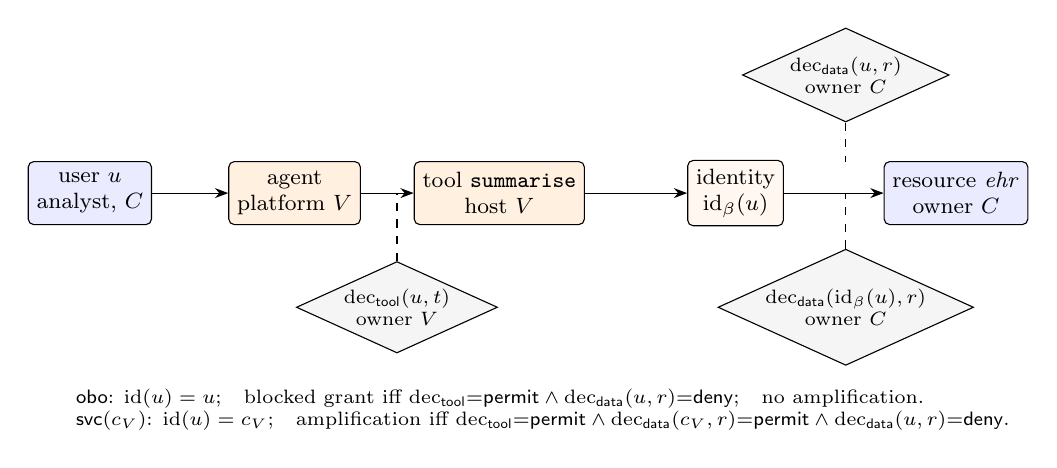
\begin{tikzpicture}[font=\footnotesize, >=Stealth,
  p/.style={draw, rounded corners=2pt, minimum height=0.8cm, align=center, inner sep=3pt},
  d/.style={draw, diamond, aspect=2.2, inner sep=0.8pt, align=center, font=\scriptsize, fill=gray!8}]
\node[p, fill=blue!8] (u) at (0,0) {user $u$\\ analyst, $C$};
\node[p, fill=orange!12] (a) at (2.6,0) {agent\\ platform $V$};
\node[p, fill=orange!12] (t) at (5.2,0) {tool \texttt{summarise}\\ host $V$};
\node[p, fill=orange!6] (i) at (8.2,0) {identity\\ $\ident_\beta(u)$};
\node[p, fill=blue!8] (r) at (11.0,0) {resource \textit{ehr}\\ owner $C$};
\draw[->] (u) -- (a); \draw[->] (a) -- (t); \draw[->] (t) -- (i); \draw[->] (i) -- (r);
\node[d] (dt) at (3.9,-1.45) {$\dec_{\mathsf{tool}}(u,t)$\\ owner $V$};
\node[d] (dd) at (9.6,-1.45) {$\dec_{\mathsf{data}}(\ident_\beta(u), r)$\\ owner $C$};
\node[d] (du) at (9.6,1.5) {$\dec_{\mathsf{data}}(u, r)$\\ owner $C$};
\draw[dashed] (dt) -- (3.9,0); \draw[dashed] (dd) -- (9.6,0); \draw[dashed] (du) -- (9.6,0.4);
\node[align=left, font=\scriptsize, anchor=west] at (-0.3,-2.75) {$\obo$: $\ident(u) = u$;\quad blocked grant iff $\dec_{\mathsf{tool}}{=}\permit \wedge \dec_{\mathsf{data}}(u,r){=}\deny$;\quad no amplification.\\
$\svc(c_V)$: $\ident(u) = c_V$;\quad amplification iff $\dec_{\mathsf{tool}}{=}\permit \wedge \dec_{\mathsf{data}}(c_V,r){=}\permit \wedge \dec_{\mathsf{data}}(u,r){=}\deny$.};
\end{tikzpicture}}
\caption{Decisions crossed by one agent call and the owners who hold them. Blocked grants and amplifications are conjunctions of decisions taken by different owners; Theorem~\ref{thm:duality} shows that switching the binding moves findings from one set to the other.}\label{fig:chain}
\end{figure}

%=====================================================================
\section{Admitting change}\label{sec:admission}

We now treat every finding as the outcome of a \emph{slot}: a pair of rules, a cross-layer cell $(u, t, r)$, a usage cell $(t, r, s)$ or $(t, r, \rho)$, or a drift cell of a tool. A state assigns each slot a finding or nothing. This section shows that an event can change only the slots of a small region, and that checking that region decides whether the invariant survives the event.

\subsection{Regions}\label{sec:region}
Let $\mathrm{rd}(r) = \{t : r \in \reads(d_1(t))\}$ be the tools that currently read $r$.

\begin{definition}[Region of an event]\label{def:region}
For a state $\G$ and an event $\epsilon$, the region $\Reg(\epsilon)$ is the following set of slots.
\begin{itemize}
\item $\mathsf{ins}(e)$ or $\mathsf{del}(e)$ with $e$ in layer $\ell$: the pairs $\{e, e'\}$ with $e'$ in layer $\ell$ and $\key(e) \cap \key(e') \neq \emptyset$, together with
\begin{itemize}
\item if $\ell = \mathsf{data}$: the cells $(u, t, r)$ with $u \in S$, $r \in \key(e)$, $t \in \mathrm{rd}(r)$;
\item if $\ell = \mathsf{tool}$: the cells $(u, t, r)$ with $u \in S$, $t \in \key(e)$, $r \in \reads(d_1(t))$;
\item if $\ell = \mathsf{usage}$: the usage and drift cells of the tools in $\mathrm{rd}(r)$, $r \in \key(e)$.
\end{itemize}
\item $\mathsf{redesc}(t, d)$: every cross-layer, usage and drift cell of $t$, for the resources of $\reads(d_1(t)) \cup \reads(d)$.
\item $\mathsf{approve}(t)$: the drift cells of $t$.
\end{itemize}
\end{definition}
The region is defined by key vertices and by the reads relation, both of which are indexed; it does not depend on the rest of the hypergraph.

\begin{theorem}[Locality]\label{thm:locality}
For every state $\G$ and event $\epsilon$, every slot outside $\Reg(\epsilon)$ has the same finding in $\G$ and in $\G \oplus \epsilon$. Consequently
\begin{equation}
\F(\G \oplus \epsilon) = \bigl(\F(\G) \setminus \Reg(\epsilon)\bigr) \cup \F_{\Reg(\epsilon)}(\G \oplus \epsilon), \label{eq:locality}
\end{equation}
where $\F_X$ denotes the findings in the slots of $X$.
\end{theorem}
\begin{proof}
\emph{Rule events.} Pairs that do not contain $e$ keep their match sets, effects and owners. A pair $\{e, e'\}$ with $\key(e) \cap \key(e') = \emptyset$ has $c(\kappa) \cap c'(\kappa) = \emptyset$ on the key attribute $\kappa$, so it neither overlaps (\Cref{lem:overlap}) nor stands in subsumption (\Cref{lem:subsume}, since $c(\kappa)$ is non-empty), and is not a finding before or after the event. By \Cref{def:rule}, $\dec_\ell(q)$ depends only on the rules matching $q$, and a rule matches a data or usage request on $r$ only if $r$ is among its key vertices, and a tool request on $t$ only if $t$ is. Hence a data event changes $\dec_{\mathsf{data}}(i, r)$ only for $r \in \key(e)$, a tool event changes $\dec_{\mathsf{tool}}(u, t)$ only for $t \in \key(e)$, and a usage event changes $\dec_{\mathsf{usage}}(r, p, s)$ only for $r \in \key(e)$. The cells of \Cref{def:cross} are conjunctions of $\dec_{\mathsf{tool}}(u, t)$ and $\dec_{\mathsf{data}}$ on the resource of the cell, so they change only in the cells listed. A usage cell of $t$ on $r$ reads $\dec_{\mathsf{usage}}$ on $r$ only. $\Drift_t$ contains only elements of $\Viol(d_1(t))$, whose resources are read by $t$; changes of $\Viol(d_0(t))$ on a resource that $d_1(t)$ does not read cannot remove any of them.
\emph{Tool events.} Every slot of \Cref{def:cross,def:usage} other than pairs is indexed by one tool and reads the description of that tool only, so $\mathsf{redesc}(t, d)$ changes only cells of $t$, and $\mathsf{approve}(t)$ only $\Drift_t$.
Equation~\eqref{eq:locality} restates the claim.
\end{proof}

\subsection{Admission}\label{sec:admit}
\begin{definition}[Admission check]\label{def:admission}
An event $\epsilon$ is \emph{admitted} in state $\G$ when $\F_{\Reg(\epsilon)}(\G \oplus \epsilon) \subseteq \Acc$. Otherwise it is \emph{held}, and the findings $\F_{\Reg(\epsilon)}(\G \oplus \epsilon) \setminus \Acc$ are sent to the owners they involve.
\end{definition}

\begin{theorem}[Admission is necessary and sufficient]\label{thm:preservation}
Let $\G$ be a governed state and $\epsilon$ an event. Then $\epsilon$ is admitted if and only if $\G \oplus \epsilon$ is governed. Consequently, if $\G_0$ is governed and only admitted events are applied, every reachable state is governed. If $\G_0$ is not governed, applying only admitted events never adds an unaccepted finding: $\F(\G \oplus \epsilon) \setminus \Acc \subseteq \F(\G) \setminus \Acc$.
\end{theorem}
\begin{proof}
By \eqref{eq:locality}, $\F(\G \oplus \epsilon) \setminus \Acc = \bigl((\F(\G) \setminus \Reg(\epsilon)) \setminus \Acc\bigr) \cup \bigl(\F_{\Reg(\epsilon)}(\G \oplus \epsilon) \setminus \Acc\bigr)$. If $\G$ is governed the first set is empty, so $\G \oplus \epsilon$ is governed exactly when the second set is empty, which is the admission condition. The second claim follows by induction on the number of events. For the third, if $\epsilon$ is admitted the second set is empty and the first is contained in $\F(\G) \setminus \Acc$.
\end{proof}
The check is thus \emph{exact}: an admitted event never breaks the invariant, and a held event always would. It does not depend on how the findings in the region are computed, which lets Section~\ref{sec:protocol} compute them on secret shares.

Owners act concurrently, so events must be admitted concurrently as well. Define the \emph{footprint} $\Phi(\epsilon)$ of an event as the vertices whose index entries its region reads or its application writes: $\key(e) \cup \bigcup_{r \in \key(e)} \mathrm{rd}(r)$ for data and usage rules, $\key(e) \cup \bigcup_{t \in \key(e)} \reads(d_1(t))$ for tool rules, and $\{t\} \cup \reads(d_1(t)) \cup \reads(d)$ for $\mathsf{redesc}(t, d)$ and $\mathsf{approve}(t)$.

\begin{proposition}[Commutation]\label{prop:commute}
If $\Phi(\epsilon_1) \cap \Phi(\epsilon_2) = \emptyset$, then the regions of $\epsilon_1$ and $\epsilon_2$ are disjoint and are the same in $\G$, $\G \oplus \epsilon_1$ and $\G \oplus \epsilon_2$, and both admission verdicts are the same in either order of application.
\end{proposition}
\begin{proof}
Every slot of $\Reg(\epsilon_i)$ contains a vertex of $\Phi(\epsilon_i)$ (a key vertex for pairs, a resource and a tool for cells), so disjoint footprints give disjoint regions. The region of $\epsilon_1$ is computed from the index entries of $\Phi(\epsilon_1)$, which $\epsilon_2$ does not write, and vice versa. By \Cref{thm:locality} applied to $\epsilon_2$, the findings of $\Reg(\epsilon_1)$ are the same in $\G \oplus \epsilon_1$ and $\G \oplus \epsilon_1 \oplus \epsilon_2$, so the verdict on $\epsilon_1$ does not depend on whether $\epsilon_2$ was applied first; symmetrically for $\epsilon_2$.
\end{proof}
Events with overlapping footprints are serialised, for instance by locking footprint vertices; in the AWS history of Section~\ref{sec:evaluation}, half of the changes touch at most \awsChangedMed{} action vertices, so conflicts between concurrent changes are rare.

\subsection{Algorithms}
Algorithm~\ref{alg:region} computes the region from two indexes: for each layer and key vertex $v$ the rules $\mathrm{Idx}_\ell[v]$ that constrain it, and for each resource the tools $\mathrm{rd}(r)$ that read it. Algorithm~\ref{alg:admit} evaluates the region in the successor state and decides. The findings of the region are kept in a store keyed by slot, so that \eqref{eq:locality} is applied by overwriting the region's entries.

\begin{algorithm}[t]
\caption{$\textsc{Region}(\epsilon)$: slots whose finding may change}\label{alg:region}
\begin{algorithmic}[1]
\Require event $\epsilon$; indexes $\mathrm{Idx}_\ell[v]$ and $\mathrm{rd}(r)$; population $S$
\Ensure candidate pairs $P$, cross-layer keys $X$, tools $T_u$ whose usage and drift cells must be re-evaluated
\State $P, X, T_u \gets \emptyset$
\If{$\epsilon = \mathsf{ins}(e)$ or $\mathsf{del}(e)$, with $e$ in layer $\ell$}
  \State $P \gets \{\{e, e'\} : v \in \key(e),\ e' \in \mathrm{Idx}_\ell[v] \setminus \{e\}\}$ \Comment{\Cref{lem:overlap,lem:subsume}}
  \If{$\ell = \mathsf{data}$} $X \gets \{(t, r) : r \in \key(e),\ t \in \mathrm{rd}(r)\}$
  \ElsIf{$\ell = \mathsf{tool}$} $X \gets \{(t, r) : t \in \key(e),\ r \in \reads(d_1(t))\}$
  \Else\ $T_u \gets \bigcup_{r \in \key(e)} \mathrm{rd}(r)$
  \EndIf
\ElsIf{$\epsilon = \mathsf{redesc}(t, d)$}
  \State $X \gets \{(t, r) : r \in \reads(d_1(t)) \cup \reads(d)\}$;\quad $T_u \gets \{t\}$
\ElsIf{$\epsilon = \mathsf{approve}(t)$}
  \State $T_u \gets \{t\}$
\EndIf
\State \Return $P$, $X \times S$ (cells $(u, t, r)$), $T_u$
\end{algorithmic}
\end{algorithm}

\begin{algorithm}[t]
\caption{$\textsc{Admit}(\epsilon)$: exact admission of one event}\label{alg:admit}
\begin{algorithmic}[1]
\Require governed state $\G$ with finding store $\mathcal{S}$ (slot $\mapsto$ finding); accepted set $\Acc$
\Ensure verdict, and findings for their owners
\State $(P, X, T_u) \gets \textsc{Region}(\epsilon)$ \Comment{Algorithm~\ref{alg:region}}
\State $\G' \gets \G \oplus \epsilon$ \Comment{tentative; indexes updated on a copy of the footprint}
\State $N \gets \emptyset$
\ForAll{$\{e, e'\} \in P$}
  \State $N \gets N \cup \textsc{PairCheck}(e, e')$ \Comment{local if one owner, else Algorithm~\ref{alg:pairsecure}}
\EndFor
\ForAll{$(t, r) \in X$}
  \State $N \gets N \cup \textsc{CellCheck}(t, r, S)$ \Comment{local if one owner, else Algorithm~\ref{alg:ldsc}}
\EndFor
\ForAll{$t \in T_u$}
  \State $N \gets N \cup \Viol(d'_1(t)) \cup \bigl(\Viol(d'_1(t)) \setminus \Viol(d'_0(t))\bigr)$ \Comment{evaluated by the owners of $\reads(t)$}
\EndFor
\If{$N \subseteq \Acc$}
  \State commit $\G'$; overwrite the entries of $P$, $X \times S$ and $T_u$ in $\mathcal{S}$ with $N$ \Comment{\eqref{eq:locality}}
  \State \Return \textsc{accept}
\Else
  \State \Return \textsc{hold}, and send each finding of $N \setminus \Acc$ to the owners it involves, ranked by Section~\ref{sec:ranking}
\EndIf
\end{algorithmic}
\end{algorithm}

\begin{proposition}[Cost]\label{prop:cost}
Let $n_v = |\mathrm{Idx}_\ell[v]|$, $m = |A_\ell|$ and $N_\ell$ the number of rules of layer $\ell$. Admitting a rule event costs $O\bigl(m \sum_{v \in \key(e)} n_v\bigr)$ pair tests and $O\bigl(|S|\,(m \sum_{v \in \key(e)} n_v + |X|)\bigr)$ for the cells, where $|X| \le |\key(e)| \cdot \max_r |\mathrm{rd}(r)|$ for data rules and $|\key(e)| \cdot \max_t |\reads(t)|$ for tool rules. Full recomputation costs $O(m \sum_v n_v^2)$ pair tests and $O\bigl(|S|(m N_\ell + \sum_t |\reads(t)|)\bigr)$ for the cells.
\end{proposition}
\begin{proof}
Each pair test is a per-attribute set comparison (\Cref{lem:overlap,lem:subsume}). A decision row $\dec_\ell(\cdot, v)$ over $S$ is recomputed from the $n_v$ rules on $v$ in $O(|S| m n_v)$, and each cell key then costs $O(|S|)$. Full recomputation does the same for every vertex and every pair inside each bucket.
\end{proof}
When rules spread over many key vertices, $n_v$ is small and the ratio between full recomputation and admission grows with the number of vertices; Section~\ref{sec:scale} measures it.

\begin{example}[Running example, admission]\label{ex:admission}
Before the three events, both clinicians and analysts form blocked grants on \texttt{summarise} and \textit{ehr}, since $C$ denies $V$'s service account; suppose $C$ and $V$ had accepted them.
\textbf{$\epsilon_1 = \mathsf{ins}(e_5)$} has $\key(e_5) = \{\textit{ehr}\}$ and $\mathrm{rd}(\textit{ehr}) = \{\texttt{summarise}\}$, so its region is the pair $\{e_5, e_3\}$ (both of $C$, checked locally) and the cells $(u, \texttt{summarise}, \textit{ehr})$. In the successor state the two blocked grants disappear and $(\textit{analyst}, \texttt{summarise}, \textit{ehr})$ becomes an amplification, as Theorem~\ref{thm:duality} predicts. The event is held, and the finding goes to $C$ and $V$.
\textbf{$\epsilon_2 = \mathsf{redesc}(\texttt{export}, d)$} has the cells of \texttt{export} as its region. The usage cell $(\texttt{export}, \textit{claims}, R/\mathrm{US})$ is denied by $C$'s usage rule and absent under the approved description: a usage violation and a drift, sent to $C$ and $V$.
\textbf{$\epsilon_3 = \mathsf{ins}(e_7)$}, a tool rule on \texttt{export}, has the cells $(u, \texttt{export}, \textit{claims})$ as its region; interns are offered \texttt{export} but $C$ denies them \textit{claims}: a blocked grant. $C$ may accept it, since the call will simply fail, or $V$ may withdraw the rule.
Figure~\ref{fig:hg}b shows the three new hyperedges and their key vertices. None of the three checks reads any rule of the hypergraph outside the region of its event.
\end{example}

%=====================================================================
\section{Admission across owners without disclosure}\label{sec:protocol}

Algorithm~\ref{alg:admit} needs, for slots whose rules belong to several owners, findings that no owner can compute alone. This section computes them on secret shares so that each owner learns the findings that involve it and nothing else beyond a stated leakage. Slots of a single owner are evaluated by that owner in the clear.

\subsection{Building blocks}\label{sec:mpcbasics}
Two servers $S_1, S_2$ hold additive shares $\shr{x} = (x_1, x_2)$ with $x = x_1 + x_2$ in $\Fp$, $p = 2^{31}-1$. Additions and multiplications by public constants are local. A product $\shr{xy}$ uses a Beaver triple $(\shr{a}, \shr{b}, \shr{ab})$ from a dealer~\cite{beaver1991triples}: the servers open $d = x - a$ and $e = y - b$ and set $\shr{xy} = \shr{ab} + d\shr{b} + e\shr{a} + de$. An input matrix $X$ is masked once by a random matrix $A$ and $X - A$ is opened; products $X Y^{\top}$ of masked inputs then need no further interaction, given shares of $A_X A_Y^{\top}$ from the dealer. Outputs are sent by both servers to the owner entitled to them, never opened to the servers.

\subsection{Same-layer pairs as inner products}\label{sec:pairsecure}
Write $\chi_a(e) \in \{0,1\}^{D_a}$ for the indicator of $c(a)$, a wildcard being the full domain, and $\chi(e)$ for the concatenation over $a \in A_\ell$. For two rules, $\langle \chi_a(e), \chi_a(e')\rangle = |c(a) \cap c'(a)|$. With $x_{ee'} = \eta_e + \eta_{e'} - 2\eta_e\eta_{e'}$, where $\eta \in \{0,1\}$ encodes the effect, \Cref{lem:overlap,lem:subsume} give
\begin{align}
e \text{ conflicts with } e' &\iff x_{ee'} \textstyle\prod_{a \in A_\ell} \langle \chi_a(e), \chi_a(e')\rangle \neq 0, \label{eq:secconf}\\
e \text{ is redundant w.r.t.\ } e' &\iff \bigl(|\chi(e)| - \langle \chi(e), \chi(e')\rangle\bigr) + x_{ee'} = 0, \label{eq:secred}
\end{align}
because $|\chi(e)| - \langle \chi(e), \chi(e')\rangle = \sum_a |c(a) \setminus c'(a)|$. Every factor is an integer smaller than $|V_\ell| + 2 < p$, so a product in $\Fp$ is zero exactly when one factor is. \Cref{fig:incidence} works the tests on three rows. Algorithm~\ref{alg:pairsecure} applies these tests to the rule $e$ of an event and the foreign rules $J$ that share a key vertex with it.


\begin{figure}[t]
\centering
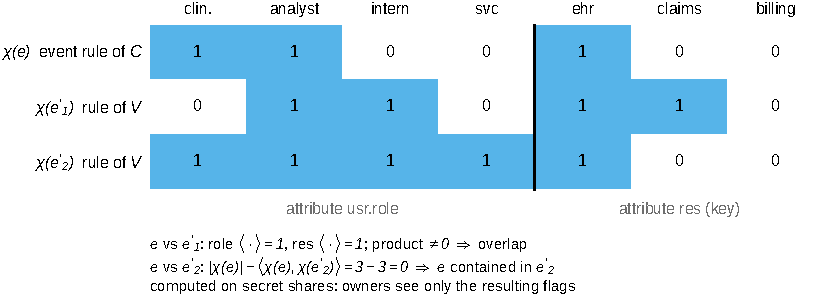
\includegraphics[width=0.85\linewidth]{figures/fig_incidence.pdf}
\caption{Incidence rows of three rules over two attributes. Per-attribute inner products give overlap, and $|\chi(e)|-\langle\chi(e),\chi(e')\rangle$ gives containment; the servers evaluate these on secret shares.}\label{fig:incidence}
\end{figure}
\begin{algorithm}[t]
\caption{$\textsc{PairSecure}(e, J)$: same-layer findings between an event's rule and foreign rules}\label{alg:pairsecure}
\begin{algorithmic}[1]
\Require rule $e$ of the event's owner; rules $J = (e'_1, \dots, e'_N)$ of other owners with $\key(e'_j) \cap \key(e) \neq \emptyset$
\Ensure to the event's owner: whether $e$ conflicts with, or is redundant w.r.t., some $e'_j$; to the owner of $e'_j$: whether $e'_j$ conflicts with $e$ or is redundant w.r.t.\ $e$
\State each owner masks and shares its rows $\chi(\cdot)$ and effects $\eta$ \Comment{one opening per input}
\State $\shr{x_j} \gets \shr{\eta_e} + \shr{\eta_j} - 2\shr{\eta_e\eta_j}$ for all $j$ \Comment{masked products, no interaction}
\State $\shr{z_j} \gets \shr{x_j}$; \textbf{for} $a \in A_\ell$ \textbf{do} $\shr{z_j} \gets \shr{z_j} \cdot \langle \shr{\chi_a(e)}, \shr{\chi_a(e'_j)}\rangle$ \Comment{$|A_\ell|$ Beaver rounds}
\State send $\sum_j \rho_j \shr{z_j}$ (random $\rho_j$) to the event's owner; send $\rho'_j \shr{z_j}$ to the owner of $e'_j$ \Comment{conflict, \eqref{eq:secconf}}
\State $\shr{w_j} \gets |\shr{\chi(e)}| - \langle \shr{\chi(e)}, \shr{\chi(e'_j)}\rangle + \shr{x_j}$ \Comment{redundancy of $e$, \eqref{eq:secred}}
\State send $\rho \prod_j \shr{w_j}$ (random $\rho \neq 0$, product by a balanced tree) to the event's owner
\State symmetrically, send $\rho''_j\bigl(|\shr{\chi(e'_j)}| - \langle \shr{\chi(e'_j)}, \shr{\chi(e)}\rangle + \shr{x_j}\bigr)$ to the owner of $e'_j$
\State each recipient reads a flag as ``value $\neq 0$'' for conflicts and ``value $= 0$'' for redundancy
\end{algorithmic}
\end{algorithm}

\subsection{Cross-layer cells: decide locally, combine securely}\label{sec:ldsc}
For a cell $(t, r)$ whose tool host $h$ differs from the owners $K_r$ of $r$, each party evaluates its \emph{own} policy in the clear and only the conjunction of \Cref{def:cross} is computed jointly. The host computes $\tau_u = [\dec_{\mathsf{tool}}(u, t) = \permit]$ for $u \in S$. Each owner $k \in K_r$ computes, for each identity $i \in S \cup \{c\}$ where $c$ is the service account of $t$ if any, $\pi_k(i) = 1$ if one of its permit rules matches $(i, r)$ and $\delta_k(i) = 1$ if one of its deny rules does. Under deny-overrides the joint decision is
\begin{equation}
D(i) = \Bigl(1 - \prod_{k \in K_r} \bigl(1 - \pi_k(i)\bigr)\Bigr) \prod_{k \in K_r} \bigl(1 - \delta_k(i)\bigr), \label{eq:jointdec}
\end{equation}
and permit-overrides is obtained by dropping the second product. When $|K_r| = 1$ the owner computes $D$ directly, for any combining function. Algorithm~\ref{alg:ldsc} then evaluates \Cref{def:cross} with one or two products per user.

\begin{algorithm}[t]
\caption{$\textsc{CellSecure}(t, r)$: decide locally, combine securely}\label{alg:ldsc}
\begin{algorithmic}[1]
\Require host $h$ of $t$ with $\tau \in \{0,1\}^{S}$; owners $K_r$ of $r$ with local bits $\pi_k, \delta_k$ on $S \cup \{c\}$
\Ensure blocked-grant and amplification flags for $(u, t, r)$, $u \in S$, to $h$ and to the owners of $r$
\State all parties share their bit vectors
\State $\shr{D} \gets$ \eqref{eq:jointdec} with $2(|K_r| - 1) + 1$ products of vectors \Comment{skipped if $|K_r| = 1$}
\If{$\beta_t = \obo$}
  \State $\shr{g_u} \gets \shr{\tau_u}(1 - \shr{D(u)})$;\quad $\shr{a_u} \gets 0$
\Else \Comment{$\beta_t = \svc(c)$}
  \State $\shr{g_u} \gets \shr{\tau_u}(1 - \shr{D(c)})$;\quad $\shr{a_u} \gets \shr{\tau_u}\shr{D(c)}(1 - \shr{D(u)})$
\EndIf
\State send $\shr{g}$ and $\shr{a}$ to the recipients (or only $\rho \sum_u \shr{g_u}$ and $\rho' \sum_u \shr{a_u}$ in \emph{existence-only} mode)
\end{algorithmic}
\end{algorithm}

Usage and drift cells need no cryptography. The owner of a resource must see the description of every tool that reads it in order to approve it; it therefore evaluates $\Viol$ and $\Drift_t$ on its own usage rules and the disclosed description, and tells the host which elements are violated.

\begin{figure}[t]
\centering
\resizebox{\linewidth}{!}{%
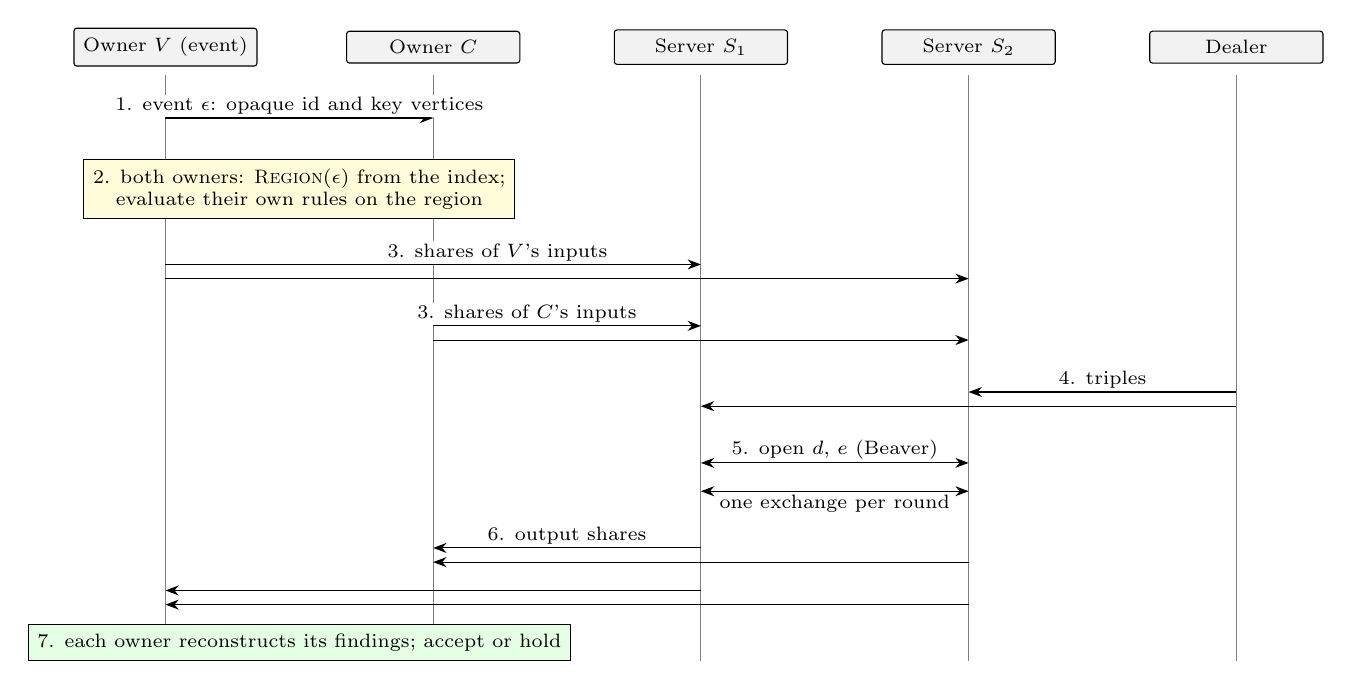
\begin{tikzpicture}[font=\scriptsize, >=Stealth, x=1cm, y=0.6cm,
  lbl/.style={fill=white, inner sep=1pt}]
\foreach \x/\n in {0/{Owner $V$ (event)},3.4/{Owner $C$},6.8/{Server $S_1$},10.2/{Server $S_2$},13.6/{Dealer}}{
  \node[draw, fill=gray!10, rounded corners=1pt, minimum width=2.2cm, align=center] at (\x,0) {\n};
  \draw[gray] (\x,-0.6) -- (\x,-13.0);}
\draw[->] (0,-1.5) -- node[lbl, above] {1. event $\epsilon$: opaque id and key vertices} (3.4,-1.5);
\node[draw, fill=yellow!15, align=center, font=\scriptsize] at (1.7,-3.0) {2. both owners: $\textsc{Region}(\epsilon)$ from the index;\\ evaluate their own rules on the region};
\draw[->] (0,-4.6) -- node[lbl, above, pos=0.62] {3. shares of $V$'s inputs} (6.8,-4.6);
\draw[->] (0,-4.9) -- (10.2,-4.9);
\draw[->] (3.4,-5.9) -- node[lbl, above, pos=0.35] {3. shares of $C$'s inputs} (6.8,-5.9);
\draw[->] (3.4,-6.2) -- (10.2,-6.2);
\draw[->] (13.6,-7.3) -- node[lbl, above] {4. triples} (10.2,-7.3);
\draw[->] (13.6,-7.6) -- (6.8,-7.6);
\draw[<->] (6.8,-8.8) -- node[lbl, above] {5. open $d$, $e$ (Beaver)} (10.2,-8.8);
\draw[<->] (6.8,-9.4) -- node[lbl, below] {one exchange per round} (10.2,-9.4);
\draw[->] (6.8,-10.6) -- node[lbl, above, pos=0.5] {6. output shares} (3.4,-10.6);
\draw[->] (10.2,-10.9) -- (3.4,-10.9);
\draw[->] (6.8,-11.5) -- (0,-11.5);
\draw[->] (10.2,-11.8) -- (0,-11.8);
\node[draw, fill=green!10, align=center, font=\scriptsize] at (1.7,-12.6) {7. each owner reconstructs its findings; accept or hold};
\end{tikzpicture}}
\caption{Message flow of one admission across two owners. Servers see only uniformly random shares and openings; each owner receives only the outputs that concern its rules, tools or resources.}\label{fig:sequence}
\end{figure}

\subsection{Security}\label{sec:security}
Let $\mathcal{F}_\epsilon$ be the functionality that receives the fragments of the owners of $\Reg(\epsilon)$ and returns to each of them the findings of the region that involve its rules, tools or resources, in the granularity of Algorithms~\ref{alg:pairsecure} and~\ref{alg:ldsc}. Let the leakage $\mathcal{L}(\epsilon)$ consist of: the key vertices of $\epsilon$ and the identifiers of the owners in its region; the number of rules each owner holds on each key vertex of the region; the population size $|S|$; the bindings of the tools in the region and, to the owner of a resource, the descriptions of the tools that read it.

\begin{theorem}[Security]\label{thm:security}
Against a semi-honest adversary that corrupts one server, or any set of owners but no server, the protocol formed by Algorithms~\ref{alg:pairsecure} and~\ref{alg:ldsc} and the local usage check computes $\mathcal{F}_\epsilon$ with leakage $\mathcal{L}(\epsilon)$: there is a simulator that, given only the corrupted parties' inputs, outputs and $\mathcal{L}(\epsilon)$, produces a view whose distribution is identical to the real view for a corrupted server and within statistical distance $q/p$ for a coalition of owners that receives $q$ conflict outputs.
\end{theorem}
\begin{proof}[Proof sketch]
We follow the simulation paradigm~\cite{goldreich2004foundations}. \emph{Corrupted server.} Its view consists of (i) one share of every input, (ii) the openings $d = x - a$, $e = y - b$ and $X - A$, and (iii) its own randomness. Shares are uniform in $\Fp$ and independent of the inputs. Each opening is the input minus a value $a$, $b$ or $A$ that is uniform and unknown to the server, since the dealer shares it and the other server does not collude; openings for distinct products use fresh triples, and a masked input is opened once and then reused only in local products. The view is therefore a vector of independent uniform elements whose length is fixed by the number of rules per key vertex, $|S|$, $|A_\ell|$ and the bindings, all of which are in $\mathcal{L}(\epsilon)$. The simulator samples such a vector. Outputs are not sent to servers.
\emph{Corrupted owners.} Their view consists of their own inputs, shares they produce, and the values sent to them. Blocked-grant and amplification bits, and the local usage results, are outputs of $\mathcal{F}_\epsilon$. A redundancy value $\rho \prod_j w_j$ with $\rho$ uniform in $\Fp^{*}$ is $0$ when the flag is set and uniform in $\Fp^{*}$ otherwise, which the simulator reproduces from the flag. A conflict value $\sum_j \rho_j z_j$ with $\rho_j$ uniform in $\Fp$ is $0$ when no $z_j \neq 0$ and uniform in $\Fp$ otherwise; the simulator outputs $0$ or a uniform element, which differs from the real distribution only by the event that a uniform element equals $0$, of probability $1/p$ per output.
\end{proof}

\begin{proposition}[Correctness]\label{prop:correct}
Algorithms~\ref{alg:pairsecure} and~\ref{alg:ldsc} return the findings of \Cref{def:pair,def:cross} exactly, except that a conflict existence flag is missed with probability at most $1/p$ per output.
\end{proposition}
\begin{proof}
By \eqref{eq:secconf}, \eqref{eq:secred} and \eqref{eq:jointdec}, each flag is a product of field elements that are integers below $p$; $\Fp$ has no zero divisors, so the product is zero exactly when a factor is. Blocked-grant and amplification bits are products of bits and are opened directly. Redundancy uses a non-zero multiplier and is exact. The conflict existence value $\sum_j \rho_j z_j$ is zero for some non-zero $(z_j)$ with probability $1/p$ over the $\rho_j$.
\end{proof}
The prototype uses $p = 2^{31}-1$ for speed; a 61-bit prime reduces the error and the statistical distance of \Cref{thm:security} to $2^{-61}$ per output at about twice the communication.

\subsection{What the findings themselves reveal}\label{sec:outputleak}
Theorem~\ref{thm:security} bounds what the protocol reveals beyond the findings, not what the findings reveal. An owner can submit events crafted to learn another owner's decisions.

\begin{proposition}[Probing]\label{prop:probe}
(i) With per-user outputs, a tool host that submits a tool rule permitting every $u \in S$ on a tool that reads $r$ on behalf of the user learns $\dec_{\mathsf{data}}(u, r)$ for all $u \in S$ from one event. (ii) With existence-only outputs, each event reveals at most one bit per output, so learning a decision row whose $|S|$ entries are independent with $\Pr[\deny] = q$ requires at least $|S| \cdot H(q)$ events in expectation, where $H$ is the binary entropy.
\end{proposition}
\begin{proof}
(i) Under $\obo$, the blocked-grant flag of $(u, t, r)$ equals $1 - D(u)$ for every $u$ with $\tau_u = 1$. (ii) An event yields one binary output; by Shannon's source coding theorem, identifying a random row requires on average at least its entropy $|S| \cdot H(q)$ in bits.
\end{proof}
Part~(i) holds for any mechanism that tells a tool host which of its users would be refused, encrypted or not; it is the price of an actionable finding. Owners choose per resource between per-user outputs and existence-only outputs with a quota of events per period, which bounds the leakage to the quota in bits. Section~\ref{sec:leakeval} measures both modes.

\subsection{Cost}\label{sec:cost}
\begin{proposition}[Communication]\label{prop:comm}
For an event rule and $N$ foreign rules on its key vertices, Algorithm~\ref{alg:pairsecure} opens $O((N+1)|V_\ell|)$ elements, performs $O(N|A_\ell|)$ Beaver products in $|A_\ell| + \lceil \log_2 N \rceil + 2$ rounds, and sends $O(N)$ output elements. For a cell with $|K_r|$ owners, Algorithm~\ref{alg:ldsc} shares $O(|S||K_r|)$ elements and performs $O(|S||K_r|)$ products in $O(|K_r|)$ rounds.
\end{proposition}
\begin{proof}
By inspection of the algorithms; the redundancy product over $N$ factors is evaluated by a balanced tree.
\end{proof}
The servers' work is linear in the region rather than in the state, as in Proposition~\ref{prop:cost}. The dealer produces triples and matrix triples whose number is of the same order; replacing it by a two-party preprocessing protocol based on oblivious transfer or homomorphic encryption removes the trusted dealer at a cost we do not measure here.

%=====================================================================
\section{Ranking held changes by expected use}\label{sec:ranking}

A busy federation holds many changes, and owners must decide which to examine first. An amplification on a resource nobody requests matters less than a blocked grant on a tool used every hour. We therefore order held changes by the expected number of requests their findings affect. This is the only learned component of \name; the admission verdict never depends on it.

\paragraph{Expected impact} For a held event with findings $N$, let $\hat\lambda(u, r)$ estimate the probability that users of class $u$ request resource $r$ in the next period. The impact of the event is
\begin{multline}
\mathrm{Imp}(\epsilon) = \sum_{(u, t, r) \in N \cap (\Gap \cup \Amp)} \hat\lambda(u, r)\\
+ \sum_{\{e, e'\} \in N \cap (\Conf \cup \Red)} \ \sum_{u \in S,\ r \in \key(e) \cap \key(e')} \hat\lambda(u, r)\, [\,(u, r) \in M(e) \cap M(e')\,], \label{eq:impact}
\end{multline}
and usage findings are weighted by the requests of the classes allowed to call the tool. Held events are presented in decreasing order of $\mathrm{Imp}$.

\paragraph{Hyperedge model} A request is the hyperedge formed by the attribute vertices of the user and the vertex of the resource. Each vertex $v$ has an embedding $z_v \in \mathbb{R}^{32}$ and each resource a bias $b_r$, and
\begin{equation}
\hat\lambda(u, r) = \sigma\Bigl(\bigl\langle \textstyle\sum_{a} z_{(a, u_a)},\ z_r \bigr\rangle + b_r\Bigr), \label{eq:scorer}
\end{equation}
trained on an organisation's own log against sampled non-requests with the logistic loss. An optional propagation step replaces each embedding by itself plus the mean of the embeddings of the vertices it co-occurs with in past requests, a single vertex--hyperedge--vertex pass in the sense of hypergraph neural networks~\cite{feng2019hgnn}.

\paragraph{Federation} Organisations share the vertex vocabulary (\Cref{as:vocab}) but not their logs. They train \eqref{eq:scorer} by federated averaging~\cite{mcmahan2017fedavg} with one local epoch per round, and the server averages each vertex's embedding over the organisations that observed that vertex, weighted by the number of observations, so that a vertex absent from an organisation's log does not dilute the others. The benefit expected from federation is specific: an organisation learns about resources and tools that are new to it but known to partners, which is the situation created by a newly shared tool. Section~\ref{sec:rankeval} tests this claim and reports that it holds only in that case. The shared updates are not protected here; combining them with secure aggregation, and measuring what they leak, is future work.

%=====================================================================
\section{Evaluation}\label{sec:evaluation}

\subsection{Questions}
\begin{description}
\item[RQ1] Is incremental admission equal to full recomputation, and do the secure checks return the plaintext findings?
\item[RQ2] On real policy changes, how large is the region of a change, and what would admission have held?
\item[RQ3] Which tools in the wild can be given a finite description of what they read?
\item[RQ4] How do admission and full recomputation scale with the number of rules and organisations?
\item[RQ5] What does admission across owners cost, compared with a full secure re-check and with an earlier sketch-based design?
\item[RQ6] How much do the findings themselves reveal under per-user and existence-only outputs?
\item[RQ7] Does federated learning improve the expected-use estimate that ranks held changes?
\end{description}

\subsection{Data and setup}\label{sec:setup}
\paragraph{AWS managed-policy history} The MAMIP repository records every version of the AWS managed IAM policies~\cite{mamip}. We replay its history from 3 November 2025, when it held \awsBasePol{} policies with \awsBaseSt{} statements, to 14 November 2026. A change event is a policy whose document differs from its previous version: \awsEvents{} events, of which \awsMod{} modify a policy and \awsAdd{} add one. Statements become rules over action vertices: action patterns are expanded against the \awsUniverse{} actions written explicitly in any version, so wildcard expansion is a lower bound, and resources and conditions are kept as canonical strings. Within a policy we report redundant pairs (same effect, action set and resources contained, conditions at least as strict) and allow/deny overlaps (shared actions, overlapping resource patterns), the latter an over-approximation on resources. For cross-policy findings we need two owners; we take the \awsAgentPol{} policies whose names identify an AI agent or assistant service (Bedrock, Amazon Q, the DevOps, security, FinOps and transform agents, and similar) as the authority of an agent, and the 11 AWS job-function policies as the authority of a person. An agent policy then amplifies a person by the actions it allows unconditionally on every resource that the job function does not allow at all, a lower bound on \Cref{def:cross} at action level. This pairing is constructed: AWS does not state that holders of a job function use these agents, and the name-based selection was not checked against service documentation.

\paragraph{Static real policies} The snapshot of 14 November 2026 holds 1,686 policies and 9,602 statements. 2,751 statements (28.7\%) are attribute sets as they stand, 2,534 (26.4\%) after expanding action patterns, and 2,790 (29.1\%) after reading equality conditions as attribute sets; 1,496 (15.6\%) carry conditions that are not sets, such as string patterns or null tests, and 31 (0.3\%) use negation. The model of Section~\ref{sec:model} therefore covers 8,054 statements (83.9\%). 4,288 statements (44.7\%) carry a condition and 87 (0.9\%) deny.

\paragraph{MCP tool schemas} The MCP Atlas Census contains \csTools{} tool records with input schemas from \csServers{} servers~\cite{mcpatlas2026}. We classify a tool as \emph{open-ended} when one of its string parameters carries code, SQL, a shell command, an expression or a URL chosen at call time, and as \emph{resource-addressed} when a parameter names a resource (identifier, path, table, bucket, repository and the like).

\paragraph{Constructed federations} No public data pairs the tool, data and usage policies of several organisations, so we generate them. Each of $K$ organisations owns 20 resources and hosts 10 tools; 10 further resources are co-owned by all. The population has 8 roles and 5 departments per organisation, $|S| = 40K$ user classes, plus one service account per organisation. Each organisation writes $n$ data rules and $n/2$ tool and usage rules; a rule constrains each subject attribute with probability 0.6 to one to three values, its key attribute to one to three owned or co-owned values, and is a permit with probability 0.8; 15\% of data rules grant service accounts. A tool reads one to three resources, each drawn from all resources of the federation with probability 0.4 and otherwise from those of its host, acts on behalf of the user with probability 0.6, and has one or two sinks. Events are drawn as 30\% data-rule, 15\% tool-rule and 8\% usage-rule insertions, 12\%, 6\% and 4\% deletions, 18\% redescriptions (half of which change only sinks or retention) and 7\% approvals. Decisions use deny-overrides. Unless stated, $K = 4$ and $n = 60$.

\paragraph{Earlier benchmarks} To compare with a sketch-based design for the same problem, we reuse its three benchmarks (Agentic, XS-ABAC and AMZ-Access; six domains, six collaboration scopes, 400 shared-scope rules per domain, five seeds), on which that design reported the false-positive rate of conflict detection and the cost of its decoder on secret shares.

\paragraph{Access logs} For RQ7 we use 32,769 real access requests of the Amazon employee access data~\cite{kaggle2013amazon}, with the eight largest business units as organisations that keep their logs private. The data have no timestamps, so past and future are a random 50/50 split per organisation; test negatives pair a user class with a resource drawn from the global popularity, so that popularity alone scores 0.5. We report AUROC over \rkSeeds{} seeds, overall and separately for resources the organisation has and has not seen.

\paragraph{Implementation} The analysis library, the secure protocol and all experiments are written in Python with NumPy; the code and the scripts that produce every number and figure are released with the paper. The secure protocol runs both servers in one process and counts every message in 4-byte field elements; it does not measure network latency and uses a non-cryptographic random generator, so it establishes correctness and communication, not deployed performance. Times are from a single process on a shared cloud virtual machine and are indicative.

\subsection{RQ1: exactness}\label{sec:exact}
On ten seeds of 300 random events each, the finding store after incremental admission equals a full recomputation after every one of the \eOneEvents{} events (\eOneMism{} mismatches). Every third event was also checked on secret shares: all \eOneSP{} same-layer checks (Algorithm~\ref{alg:pairsecure}, both directions) and all \eOneSC{} cross-layer cells with several owners (Algorithm~\ref{alg:ldsc}) returned exactly the plaintext findings. On the earlier benchmarks, the secret-shared pairwise checks returned the pooled oracle's conflicts, redundancies and gaps on all \exactRuns{} runs. Property tests compare the lemmas, the duality, attenuation and incremental maintenance with brute force on 3,000 random instances, and the coNP reduction on 2,000 random formulas. On the AWS history, no within-policy finding appeared or disappeared outside the changed statements in any of the \awsEvents{} events (\awsLocViol{} violations of \Cref{thm:locality}).

\subsection{RQ2: one year of real policy changes}\label{sec:aws}
\Cref{fig:aws} and \Cref{tab:aws} summarise the replay. Changes are frequent, about three a day, and they mostly grant: \awsGain{} events add actions, \awsMut{} of them state-changing ones, while only \awsLose{} remove any.

\begin{figure}[t]
\centering
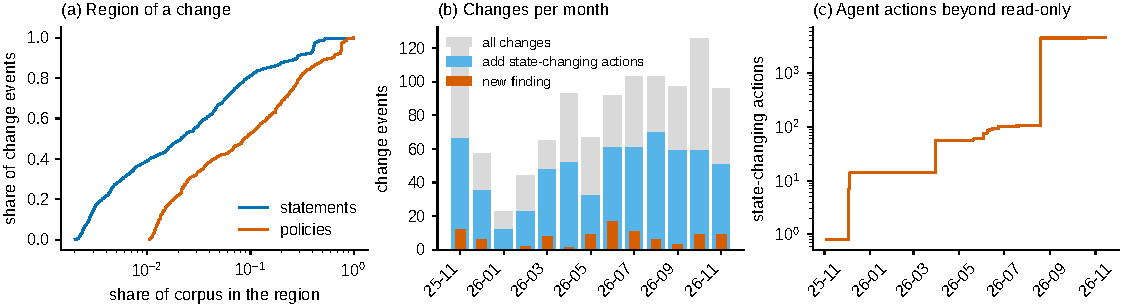
\includegraphics[width=\linewidth]{figures/fig_aws.pdf}
\caption{One year of AWS managed-policy changes replayed as events. (a) Distribution of the region of a change: share of all statements and of all policies that share an action vertex with a changed statement. (b) Changes per month, changes that add state-changing actions, and changes that introduce a finding. (c) Cumulative state-changing actions that agent-facing policies hold beyond the \texttt{ReadOnlyAccess} job function, counted at the change that introduced them.}\label{fig:aws}
\end{figure}

\begin{table}[t]
\centering\small
\caption{AWS managed-policy history, 3 November 2025 to 14 November 2026.}\label{tab:aws}
\begin{tabularx}{\linewidth}{Xr}
\toprule
Change events (modified / new policies) & \awsEvents{} (\awsMod{} / \awsAdd{})\\
Region, share of statements: median / mean / 90th percentile & \awsRegMed\% / \awsRegMean\% / \awsRegNinety\%\\
Events whose region holds under 1\% / under 5\% of statements & \awsRegUnderOne\% / \awsRegUnderFive\%\\
Region, share of policies: median / 90th percentile & \awsPolMed\% / \awsPolNinety\%\\
Findings changed outside the region & \awsLocViol\\
Events adding redundant pairs (pairs) & \awsRedEv{} (\awsRedPairs)\\
Events adding allow/deny overlaps (pairs) & \awsOvEv{} (\awsOvPairs)\\
Events on agent-facing policies / on job functions & \awsAgentEv{} / \awsJobEv\\
Agent events enlarging the amplification over some job function & \awsAmpEv\\
Agent events adding state-changing actions beyond \texttt{ReadOnlyAccess} (actions) & \awsAmpROEv{} (\awsAmpROAct)\\
Agent events adding state-changing actions beyond \texttt{ViewOnlyAccess} & \awsAmpVOEv\\
Events held by admission (any of the above findings) & \awsHeld{} (\awsHeldPct\%)\\
Admission time per event: median / 99th percentile & \awsIncMs~ms / \awsIncNinetyNine~ms\\
\bottomrule
\end{tabularx}
\end{table}

\paragraph{Locality} The region of a change is small for most changes: a median of \awsRegMed\% of statements and \awsPolMed\% of policies, and under 1\% of statements for \awsRegUnderOne\% of the events. The distribution has a long tail (\Cref{fig:aws}a): a change that writes a service-wide or global wildcard touches every statement on those actions, up to \awsRegMax\% of the corpus. Such changes are exactly the ones that deserve review, and their region is still computed from the index without reading the rest of the corpus.

\paragraph{What admission would have held} Admission would have held \awsHeld{} of the \awsEvents{} changes (\awsHeldPct\%). Inside policies, \awsRedEv{} changes introduced \awsRedPairs{} redundant statement pairs and \awsOvEv{} introduced allow/deny overlaps. Across our constructed pairing of agents and people, \awsAmpEv{} of the \awsAgentEv{} changes to agent-facing policies enlarged what an agent holds beyond some job function, and \awsAmpROEv{} of them gave the agent state-changing actions that a holder of \texttt{ReadOnlyAccess} does not have, \awsAmpROAct{} actions in total (\Cref{fig:aws}c). One change dominates: the modification of \texttt{\awsTopPol} on \awsTopDate{} added 12,202 actions, \awsTopAct{} of them state-changing and absent from \texttt{ReadOnlyAccess}. Whether this is intended is for the owners to decide; the point is that the change is visible at the moment it is made, with the affected job functions named. Changes to job-function policies, by contrast, almost never enlarged an amplification (one of \awsJobEv{} events), because they mostly add read actions.

\paragraph{Caveats} Allow/deny overlaps over-approximate resource overlap, so the \awsOvPairs{} overlap pairs are candidates; redundancy is exact for the syntactic containment we test. The amplification counts are lower bounds at action level for a pairing we constructed.

\subsection{RQ3: what tools let owners declare}\label{sec:census}
Of the \csTools{} tools, \csOpen{} (\csOpenPct\%) are open-ended: what they read is chosen at call time, so no finite $\reads(t)$ can be declared in advance, and \csSrvOpen{} servers (\csSrvOpenPct\%) expose at least one such tool. \csRes{} tools (\csResPct\%) name the resource they act on, so their reads can be declared at the granularity of a resource type. For open-ended tools the only sound description is everything the tool's identity may read; amplification is then computed on that over-approximation and blocked grants cannot be predicted. The classification is syntactic: a parameter named \texttt{url} that only selects a page of a known site is counted as open-ended, so the share is an upper estimate.

\subsection{RQ4: scaling}\label{sec:scale}
\Cref{tab:scale} and \Cref{fig:scaling} compare admission with full recomputation of all findings, over three seeds and 200 events per configuration. Full recomputation grows roughly with the square of the number of rules on each key vertex; admission grows with the rules on the event's key vertices only. At \scBigRules{} rules, recomputation takes \scBigFull~s and admission \scBigMed~ms in the median (\scBigPnn~ms at the 99th percentile), a ratio of \scBigSpeed{} on mean times, and the region holds \scBigReg\% of all slots in the median. With more organisations at fixed rules per organisation, the median admission time grows slowly, from 0.5 to 1.5~ms between 2 and 16 organisations, because each event touches the rules on a few key vertices; the 99th percentile grows faster, driven by events on co-owned resources, whose rules come from every organisation.

\begin{table}[t]
\centering\small
\caption{Admission against full recomputation on constructed federations (means over three seeds; 200 events each). Slots: rule pairs sharing a key vertex, cross-layer cells and usage cells. Speed-up: full time over mean admission time.}\label{tab:scale}
\resizebox{\linewidth}{!}{%
\begin{tabular}{rrrrrrrrr}
\toprule
$K$ & rules/org & rules & slots & full (s) & median (ms) & p99 (ms) & speed-up & region (\%)\\
\midrule
\csname @@input\endcsname generated/tab_scale 
\bottomrule
\end{tabular}}
\end{table}

\begin{figure}[t]
\centering
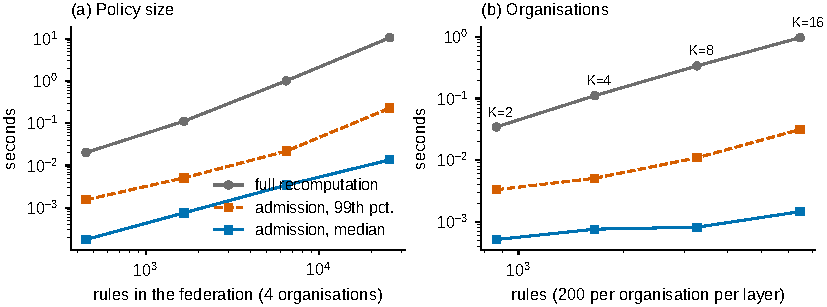
\includegraphics[width=0.98\linewidth]{figures/fig_scaling.pdf}
\caption{Time of full recomputation and of admission per event (median and 99th percentile), (a) as the number of rules grows with four organisations, (b) as the number of organisations grows with 200 rules per organisation per layer. Log--log scales.}\label{fig:scaling}
\end{figure}

\paragraph{What admission holds in the constructed federations} \Cref{tab:held} shows, per event type, the share of events that introduce each kind of finding. Redescriptions are held most often (89\%), mostly for usage violations and drift; tool-rule insertions for blocked grants and amplifications; data- and usage-rule insertions for conflicts with co-owners. Approvals never introduce a finding, since they can only remove drift. Overall \heldAll\% of events would be held. This rate reflects the random generator rather than practice, as the AWS history shows (\awsHeldPct\%); its role here is to exercise every branch of the admission check.

\begin{table}[t]
\centering\small
\caption{Share of events (\%) that introduce at least one finding of each type, by event type (ten seeds, \eOneEvents{} events).}\label{tab:held}
\resizebox{\linewidth}{!}{%
\begin{tabular}{lrrrrrrrr}
\toprule
Event & $n$ & Conf & Red & Gap & Amp & Viol & Drift & any\\
\midrule
\csname @@input\endcsname generated/tab_held 
\bottomrule
\end{tabular}}
\end{table}

\subsection{RQ5: cost across owners}\label{sec:costeval}
\Cref{tab:secure} reports the communication of admission on secret shares, against a secure re-check of the whole state. With four organisations and 1,643 rules, a full secure re-check exchanges \secMidFull~MB, while an event costs \secMidMed~kB in the median and \secMidMean~kB on average. With eight organisations and 3,237 rules, the full re-check costs \secBigFull~MB and an event \secBigMean~kB on average (\secBigPnf~kB at the 95th percentile); the tail comes from rule events on co-owned resources, whose cells involve every organisation. Most events need a single round of interaction in the median, because their only cross-owner work is one cell with one owner per side. On the AWS history, the flags-only amplification check of an agent or job-function change costs \awsSecKBMed~kB in the median under a comparable accounting (40 bytes per secure product: input sharing, Beaver opening and output), against \awsSecFullMBMed~MB for re-checking all actions; the largest change, which writes a near-global pattern, costs \awsSecMBMax~MB.

\begin{table}[t]
\centering\small
\caption{Communication of admission across owners on constructed federations (100 events each): full secure re-check of the state against one event. kB and MB of $10^3$ and $10^6$ bytes; ratio: full re-check over mean event.}\label{tab:secure}
\resizebox{\linewidth}{!}{%
\begin{tabular}{rrrrrrrrr}
\toprule
$K$ & rules & full (MB) & full rounds & median (kB) & mean (kB) & p95 (kB) & median rounds & ratio\\
\midrule
\csname @@input\endcsname generated/tab_secure 
\bottomrule
\end{tabular}}
\end{table}

\paragraph{Comparison with a sketch-based design} An alternative design summarises each domain's rules in hashed per-vertex counts and decodes anomalies from the sums of the other domains. Its decoder can also be run on secret shares. \Cref{tab:static} compares it with the exact checks of Algorithm~\ref{alg:pairsecure} on the same benchmarks, for a static analysis of all rules. The exact checks have no false alarms and cost less communication than the sketch at either size; the sketch with 512 bins falsely flags 12--55\% of non-conflicting rules, and with 4,096 bins its cost is about 30 times that of the exact checks. In its plain form, without secret sharing, the sketch also lets the other members of a scope reconstruct 66\% (512 bins) to 95\% (4,096 bins) of a domain's rules; the exact checks reveal only flags. Pooling all rules at a trusted auditor remains the cheapest exact option, at the price of disclosing every rule to it.

\begin{table}[t]
\centering\small
\caption{Static cross-domain analysis on three benchmarks (2,400 rules, six domains): sketch decoder on secret shares at 512 and 4,096 bins against the exact secret-shared checks. FPR: false-positive rate of conflict detection; MB: online communication between servers per domain (16 bytes per Beaver product); s: local computation per domain.}\label{tab:static}
\resizebox{\linewidth}{!}{%
\begin{tabular}{lrrrrrrr}
\toprule
& \multicolumn{2}{c}{Sketch, $B = 512$} & \multicolumn{2}{c}{Sketch, $B = 4096$} & \multicolumn{3}{c}{Exact (this work)}\\
\cmidrule(lr){2-3}\cmidrule(lr){4-5}\cmidrule(lr){6-8}
Benchmark & FPR & MB & FPR & MB & FPR & MB & s\\
\midrule
\csname @@input\endcsname generated/tab_static 
\bottomrule
\end{tabular}}
\end{table}

\subsection{RQ6: what the findings reveal}\label{sec:leakeval}
For each of the \leakRes{} resources of a constructed federation with \leakClasses{} user classes, we measure the events a tool host needs to learn the owner's decision row on that resource. With per-user outputs one event suffices, as Proposition~\ref{prop:probe}(i) states. With existence-only outputs and adaptive group testing by binary splitting, the host needs on average \leakProbes{} events, against an information-theoretic minimum of about \leakEntropy{} bits per row; rows are dense here (on average \leakDenied{} of \leakClasses{} classes denied), which makes splitting less efficient than asking class by class. A quota of $Q$ events per period therefore bounds the leakage to $Q$ bits, and owners that need per-user findings accept that a partner learns which of its users are refused.

\subsection{RQ7: ranking by expected use}\label{sec:rankeval}
\Cref{tab:rank} and \Cref{fig:rank} report the expected-use estimate behind \eqref{eq:impact}. The federated hyperedge model reaches AUROC \rkFed, against \rkCount{} for the best local method, simple exercise counts, so the overall gain is small. The gain is concentrated where federation can help: on resources new to the organisation, local methods are at chance (0.500), while the federated model reaches \rkFedNew. On resources the organisation already knows, federation adds nothing (\rkFedSeen{} against the same model's local 0.727). The federated model stays 0.07 below pooling all logs (\rkPool), and the propagation step does not help (\rkProp{} federated). We therefore use the model only to order held changes, and only claim benefit for tools and resources that are new to an organisation.

\begin{table}[t]
\centering\small
\caption{Expected-use estimation on real access requests (AUROC; mean over organisations and \rkSeeds{} seeds; ``new'': resources absent from the organisation's past log). Pooled: all logs at one place, an upper bound that discloses them.}\label{tab:rank}
\resizebox{\linewidth}{!}{%
\begin{tabular}{lrrrrrr}
\toprule
& \multicolumn{2}{c}{Local} & \multicolumn{2}{c}{Federated} & \multicolumn{2}{c}{Pooled}\\
\cmidrule(lr){2-3}\cmidrule(lr){4-5}\cmidrule(lr){6-7}
Model & all & new & all & new & all & new\\
\midrule
\csname @@input\endcsname generated/tab_rank 
\bottomrule
\end{tabular}}
\end{table}

\begin{figure}[t]
\centering
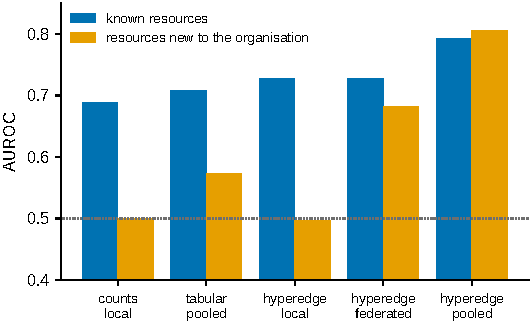
\includegraphics[width=0.62\linewidth]{figures/fig_rank.pdf}
\caption{AUROC of expected-use estimation on known resources and on resources new to the organisation.}\label{fig:rank}
\end{figure}

%=====================================================================
\section{Discussion}\label{sec:discussion}

\paragraph{What the results support} The central claims are exact and verified: a change alters findings only inside its region (\Cref{thm:locality}, no exception in \eOneEvents{} constructed and \awsEvents{} real events), checking that region is necessary and sufficient for the invariant (\Cref{thm:preservation}), and the secure checks return exactly the plaintext findings. The empirical claims are about cost and relevance: on real policy changes the region is small for most changes, and admission would have surfaced a year's growth of agent authority beyond read-only job functions at the moment each change was made.

\paragraph{Why a hypergraph, federated and dynamic} Each word names a property the method uses. The hypergraph gives one representation for rules of three layers, tool descriptions and requests, and its incidence rows turn overlap and subsumption into inner products, which is what makes the secure checks cheap. Federation is required because the findings that matter join rules of different owners. Dynamics is the object of the analysis: the region of an event is defined on the hypergraph's vertices, and the invariant is maintained event by event. Learning is confined to ranking, where it helps only for resources new to an organisation; we do not claim more.

\paragraph{Deployment} Admission fits where policy changes already pass a gate: a pull request on policy-as-code, the approval of a tool in a registry, or the publication of a new tool description at an MCP gateway. The owner's gate calls Algorithm~\ref{alg:admit} and blocks the merge or the approval while the event is held. The two servers can be run by two independent auditors, by a consortium operator and an auditor, or, when only two organisations are involved, by the two organisations themselves; the last case is ordinary two-party computation with a dealer, but \Cref{thm:security} as stated assumes that no server colludes with an owner, and we have not proved the stronger statement this deployment needs. The baseline we compare admission with is full recomputation by the same exact engine, because no existing analyser handles a federated multi-layer state; single-policy analysers such as Zelkova or Cedar's analyser~\cite{backes2018zelkova,cutler2024cedar} could serve as the local engine of each owner.

\paragraph{Limitations}
\begin{itemize}
\item \emph{Constructed cross-organisation data.} No public dataset pairs the tool, data and usage policies of several organisations. The AWS history is real but has one owner, and its agent--person pairing is ours; the federations are generated. The finding rates of the federations are not estimates of practice.
\item \emph{Vocabulary.} \Cref{as:vocab} is strong. Organisations rarely share role names or resource classes, and a mapping between vocabularies is itself a policy that can be wrong. A change to the mapping is an event whose region is every rule on the mapped vertices; we have not evaluated such events.
\item \emph{Descriptions.} Findings are relative to declared descriptions. Open-ended tools, \csOpenPct\% of the census, admit only over-approximate descriptions, and descriptions that misrepresent the code are a matter for runtime monitoring and attestation.
\item \emph{Expressiveness.} Conditions that are not attribute sets, 15.6\% of real AWS statements, are not analysed, and redundancy is tested against single rules, not unions (\Cref{thm:hard}).
\item \emph{Security model.} Semi-honest parties, two non-colluding servers and a dealer. A malicious owner could submit malformed rows to force or hide flags, and the prototype's generator and 31-bit field are not production choices. The cost of replacing the dealer was not measured, and network latency was not measured.
\item \emph{Output leakage.} Per-user findings tell a tool host which of its users a partner refuses (\Cref{prop:probe}); existence-only outputs with a quota limit this to one bit per event but are less actionable.
\item \emph{Ranking.} The learning experiment uses a random split of logs without timestamps, one dataset, and unprotected model updates.
\end{itemize}

\paragraph{Future work} The next steps are a vocabulary-mapping event with its own region, a maliciously secure variant with input validation, a dealer-free preprocessing, evaluation on time-ordered logs, and a field study with organisations that share agents and tools.

%=====================================================================
\section{Conclusion}\label{sec:conclusion}
Agents and tools make every call cross the policies of several owners, and those policies change daily. \name{} turns the question ``is the joint policy correct?'', which no owner can ask, into ``does this change keep it governed?'', which the owners concerned can answer together. The answer is exact, local and private: a change can only alter findings in a region fixed by the vertices it touches, checking that region is necessary and sufficient for the invariant, and the check runs on secret shares so that each owner learns only what concerns it. On a year of real AWS policy changes the region is a median \awsRegMed\% of statements and admission would have held \awsHeld{} changes, including those that gave agent services state-changing actions beyond read-only job functions.

\section*{CRediT authorship contribution statement}
\textbf{Mokhtar Sellami:} Conceptualization, Methodology, Software, Formal analysis, Investigation, Writing -- original draft, Writing -- review \& editing.

\section*{Declaration of competing interest}
The author declares no known competing financial interests or personal relationships that could have appeared to influence the work reported in this paper.

\section*{Declaration of generative AI and AI-assisted technologies in the manuscript preparation process}
During the preparation of this work the author used an AI assistant (Claude, Anthropic) to draft text, write and run experiment code, and check proofs. The author reviewed and edited the content and takes full responsibility for the content of the publication.

\section*{Data availability}
The AWS managed-policy history and the MCP Atlas Census are public~\cite{mamip,mcpatlas2026}; the Amazon access data are public~\cite{kaggle2013amazon}. The code that generates the constructed federations and every number, table and figure of this paper is available at \url{https://github.com/msellamiTN/DyFHL-PA}.


\bibliographystyle{elsarticle-num}
\bibliography{references}
\end{document}
